\chapter{Упражнения по работе с пользовательскими функциями \unf}

Освоить работу с расчетными функциями \unf{} можно выполняя упражнения описанные в данном разделе и изучая устройство тестовых расчетных модулей. Упражнения демонстрируют некоторые типовые приемы работы с пользовательскими функциями \unf{}. На основе этих приемов можно создать свои расчетные модули решающие специфические задачи пользователя. Примеры не являются исчерпывающими. Варианты работы с расчетными модулями \unf{} не ограничиваются описанными приемами. Цель данного описания - помочь сделать первые шаги в проведении расчетов.
Упражнения помогут: 
\begin{itemize}	
	\item 	освоить принципы работы c пользовательскими функциями \unf{} 
	\item 	изучить основы проведения инженерных расчетов в области добычи нефти
\end{itemize}

\section{Трюки и лайфхаки при работе в excel с функциями \unf{}}
Знание некоторых трюков может сильно упростить работу с пользовательскими функциями \unf{}.
\begin{enumerate}
	\item Для работы с примером должна быть запущена надстройка \unf{}. Убедиться, что надстройка запущена можно найдя вкладку Unifloc в панели меню Excel, рис. \ref{ris:excel_unifloc_tab}.
	
	\begin{figure}[h!]
		\center{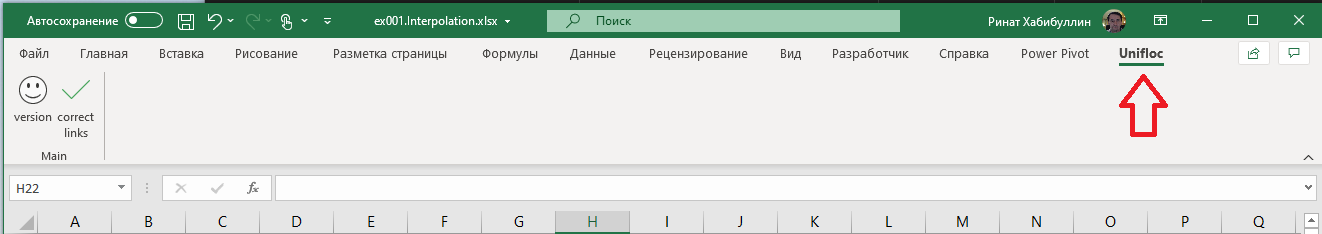
\includegraphics[width=0.8\linewidth]{excel_unifloc_tab}}
		\caption{Открытая панель Unifloc}
		\label{ris:excel_unifloc_tab}
	\end{figure}
	
	\item При необходимости вывести массив значений как результат расчета функций \mintinline{vb.net}{crv_solve} или \mintinline{vb.net}{crv_intersection} используйте комбинацию клавиш \texttt{Cntrl+Shift+Enter} или динамические массивы\footnote{подробнее про динамические массивы (dynamic arrays) можно посмотреть в интернете, например - https://www.planetaexcel.ru/techniques/2/9112/}(для новых версий Excel). Если для динамических массивов требуется подавить вывод массива - используйте знак @ в строке вызова, например как \mintinline{vb.net}{=@crv_solve(...)}.
	
	\item Все названия функций \unf{} начинаются с префикса. Это позволяет быстро искать необходимые функции. При запущенной надстройке достаточно начать вводить в ячейку формулу, например ввести \texttt{=PVT} как Excel откроет выпадающий список с подсказкой, показывающий возможные варианты названий функций (смотри рис. \ref{ris:Ex10_2}). 
	
	\begin{figure}[h!]
		\center{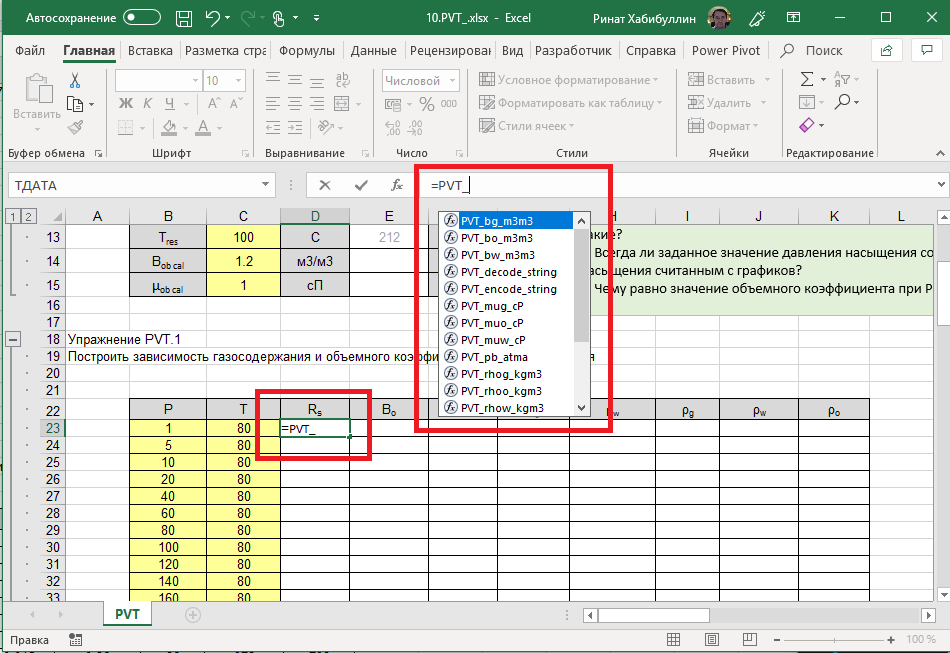
\includegraphics[width=0.8\linewidth]{Ex10_2}}
		\caption{Выпадающий список с подсказками названий функции}
		\label{ris:Ex10_2}
	\end{figure}
	
	\item 	Из выпадающего списка выберите функцию \texttt{=PVT\_Rs\_m3m3(} после чего нажмите кнопку $f_x$ "вставить функцию"  слева от строки формул. Это вызовет окно задания параметров функции, в котором будут указаны все параметры, которые необходимо ввести (смотри рис. \ref{ris:Ex10_3}). В этом окно можно задать необходимые значения параметров или указать ссылки на соответствующие ячейки. Для "хороших" функций в окне задания параметров функции будут подсказки. Также в окне задания параметров можно сразу видеть результат расчета если задан достаточный набор параметров.
	
	\begin{figure}[h!]
		\center{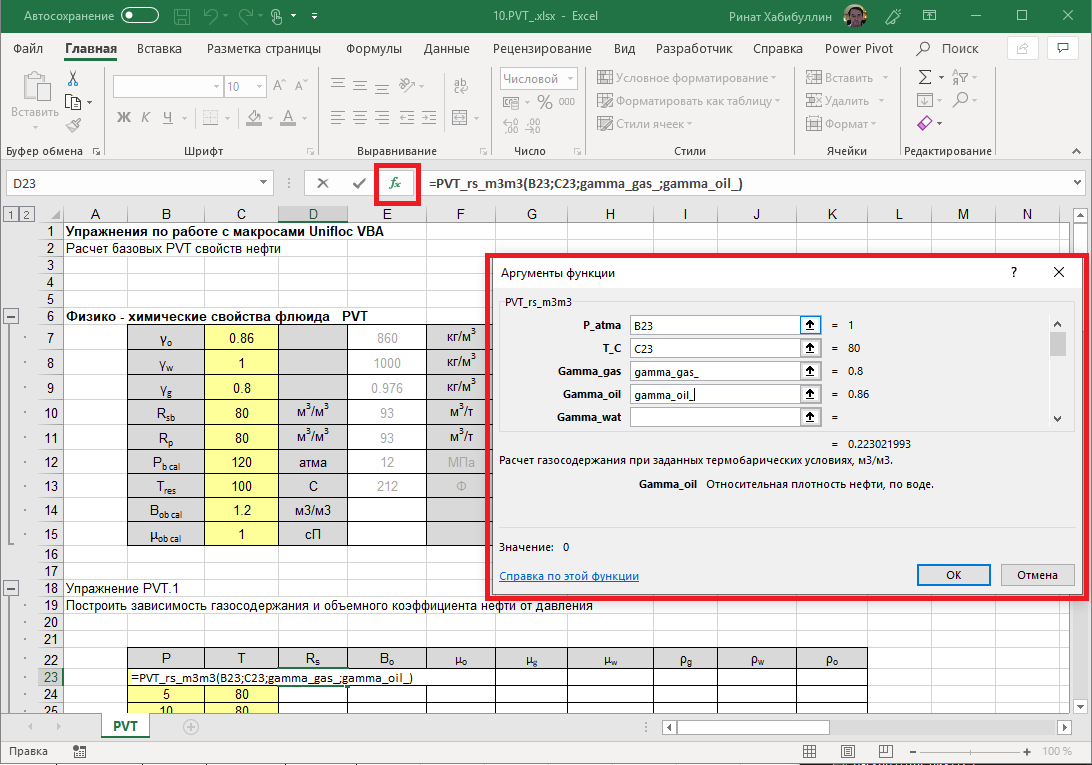
\includegraphics[width=0.8\linewidth]{Ex10_3}}
		\caption{Окно ввода аргументов функции}
		\label{ris:Ex10_3}
	\end{figure}
	
	\item После ввода всех параметров и нажатия кнопки ОК в ячейке должен отобразиться результат расчета. Воспользовавшись инструментом "Влияющие ячейки" на вкладке "Формулы"\ можно отследить на какие ячейки ссылается введенная формула (смотри рис. \ref{ris:Ex10_4})
	\begin{figure}[h!]
		\center{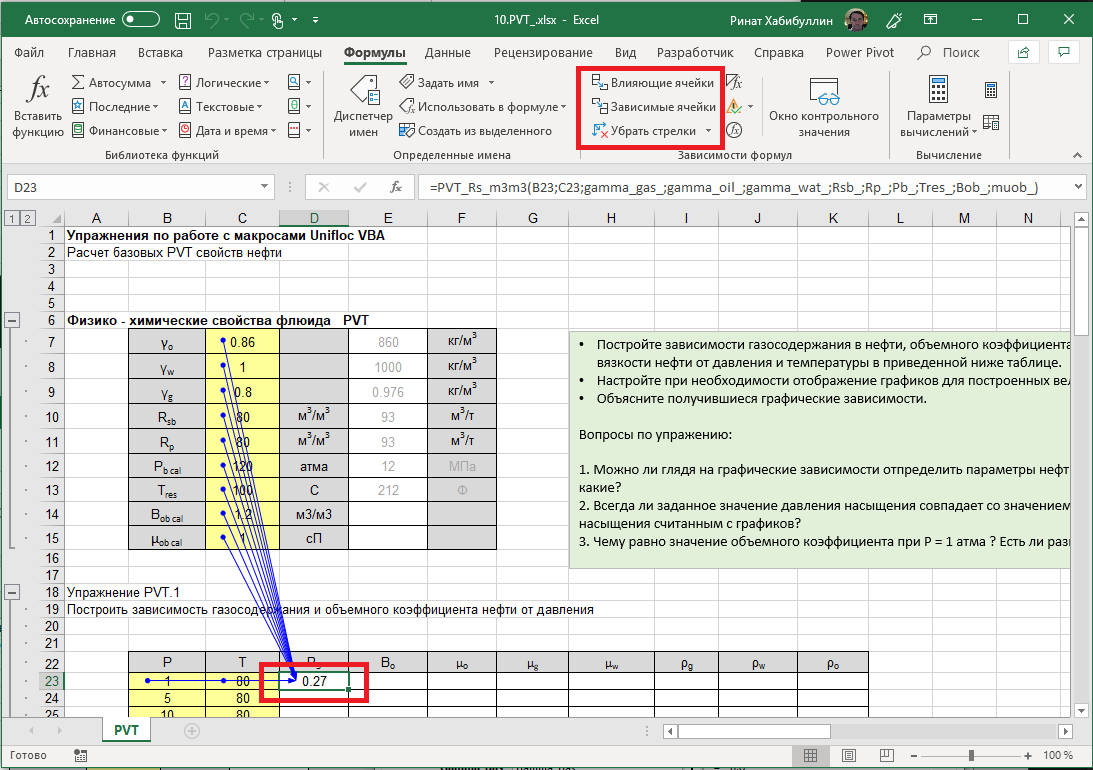
\includegraphics[width=0.8\linewidth]{Ex10_4}}
		\caption{Результат вызова пользовательской функции с отображение влияющих ячеек}
		\label{ris:Ex10_4}
	\end{figure}
\end{enumerate}


\section{Работа с таблично заданными кривыми}
Инженерный анализ требует умения ловко работать с графическими данными - кривыми, картами, кросс плотами и графиками. Кроме отображения графических данных, что легко делается стандартными программами - часто требует проводить по ним расчеты. Набор функций \unf{} для работы с таблично заданными кривыми может оказать полезными для этих целей. 

Функции \unf{} для работы с таблично заданными кривыми начинаются с префикса \mintinline{vb.net}{crv_}, от слова curve. Доступна функциональность
\begin{itemize}	
	\item интерполяции различными методами (работает и экстраполяция)
	\item поиска решения уравнения вида $f(x) = с$ где функция $f(x)$ задана таблицей (ищется решение для линейной аппроксимации)
	\item поиска пересечений двух кривых заданных таблицами (ищется решение для линейно аппроксимации)	
\end{itemize}
В коде можно обнаружить еще ряд функций, но они не будут описываться в данном руководстве, хотя по ним можно найти примеры в папке \texttt{examples} репозитория.

\subsection{Интерполяция линейная и сплайнами}
Файл примера \texttt{ex001.Interpolation.xlsx} можно найти в папке \texttt{exercises} репозитория \unf{}.

\begin{enumerate}
	\item Для работы с примером должна быть запущена надстройка \unf{}. Убедиться, что надстройка запущена можно найдя вкладку Unifloc в панели меню Excel, рис. \ref{ris:excel_unifloc_tab}.
	

	
	\item Откройте файл с упражнением \texttt{ex001.Interpolation.xlsx} (смотри рис. \ref{ris:Ex001_1}).
	
	\begin{figure}[h!]
		\center{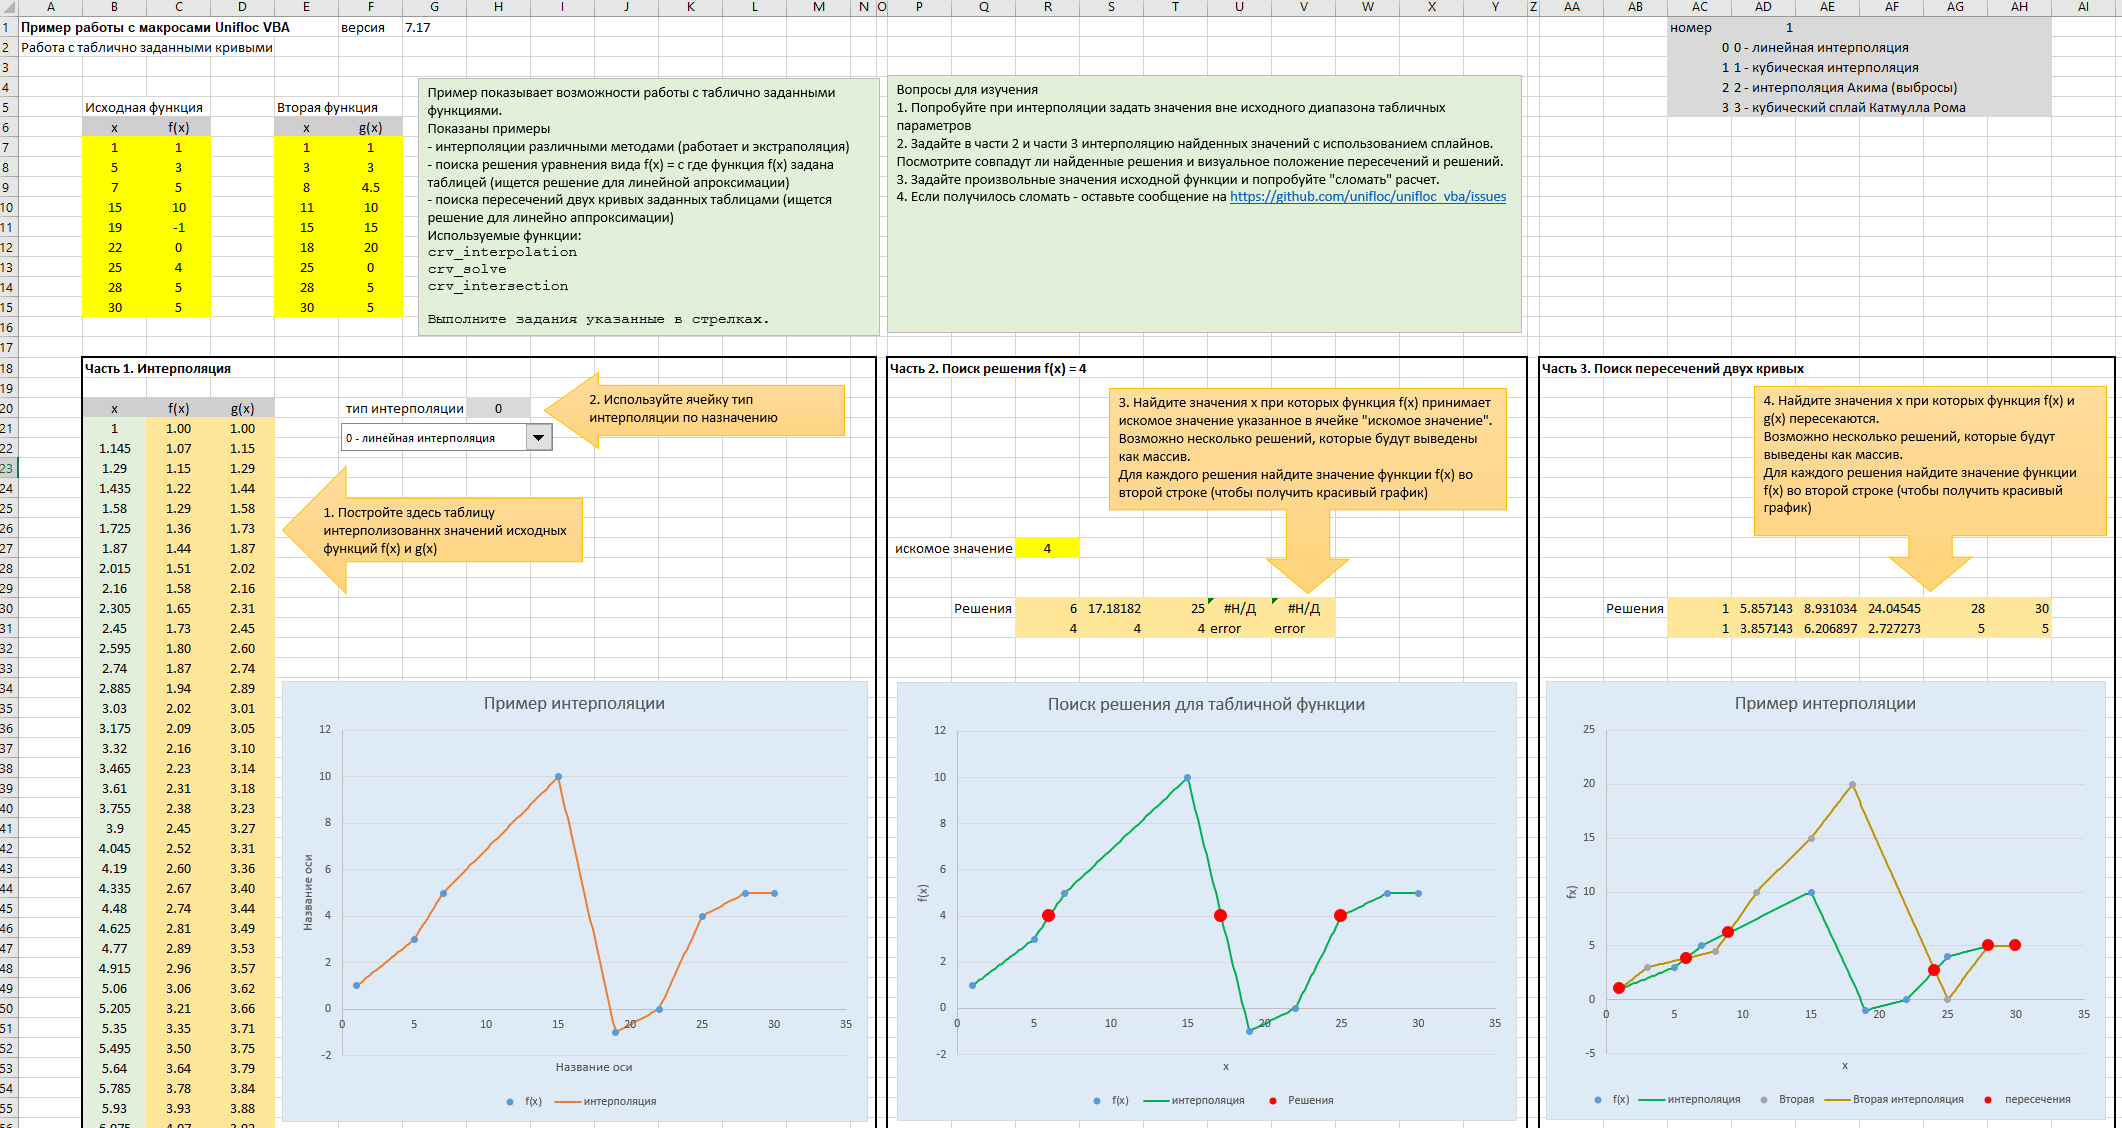
\includegraphics[width=1\linewidth]{Ex001_1}}
		\caption{Упражнение \texttt{ex001.Interpolation.xlsx} со всеми заполненными полями}
		\label{ris:Ex001_1}
	\end{figure}
	
	Пример разделен на три части: Часть 1. Интерполяция; Часть 2. Поиска решения $f(x)=c$; Часть 3.Поиск пересечения двух кривых.
	
	\item Выполните задания указанные в стрелках (последовательность выполнения по номерам стрелок). При этом должны автоматически построиться графики как на рисунке \ref{ris:Ex001_1}).
	

	
	\item Постарайтесь ответить на вопросы в блоке "Вопросы для изучения"

\end{enumerate}

\section{Расчет базовых PVT свойств флюидов}

Расчет физико химических свойств пластовых флюидов (PVT параметров) лежит в основе всех расчетов систем нефтедобычи. При решении прикладных задач редко возникает необходимость расчета PVT свойств непосредственно, однако понимание принципа их расчета, а особенно зависимости результатов расчета от исходных данных важно.
   
Для выполнения упражнения используйте файл "ex010.PVT.xlsx"

\begin{enumerate}

	\item Откройте файл с упражнением \texttt{10.PVT.xlsx} (смотри рис. \ref{ris:Ex10_1}).
	
	\begin{figure}[h!]
		\center{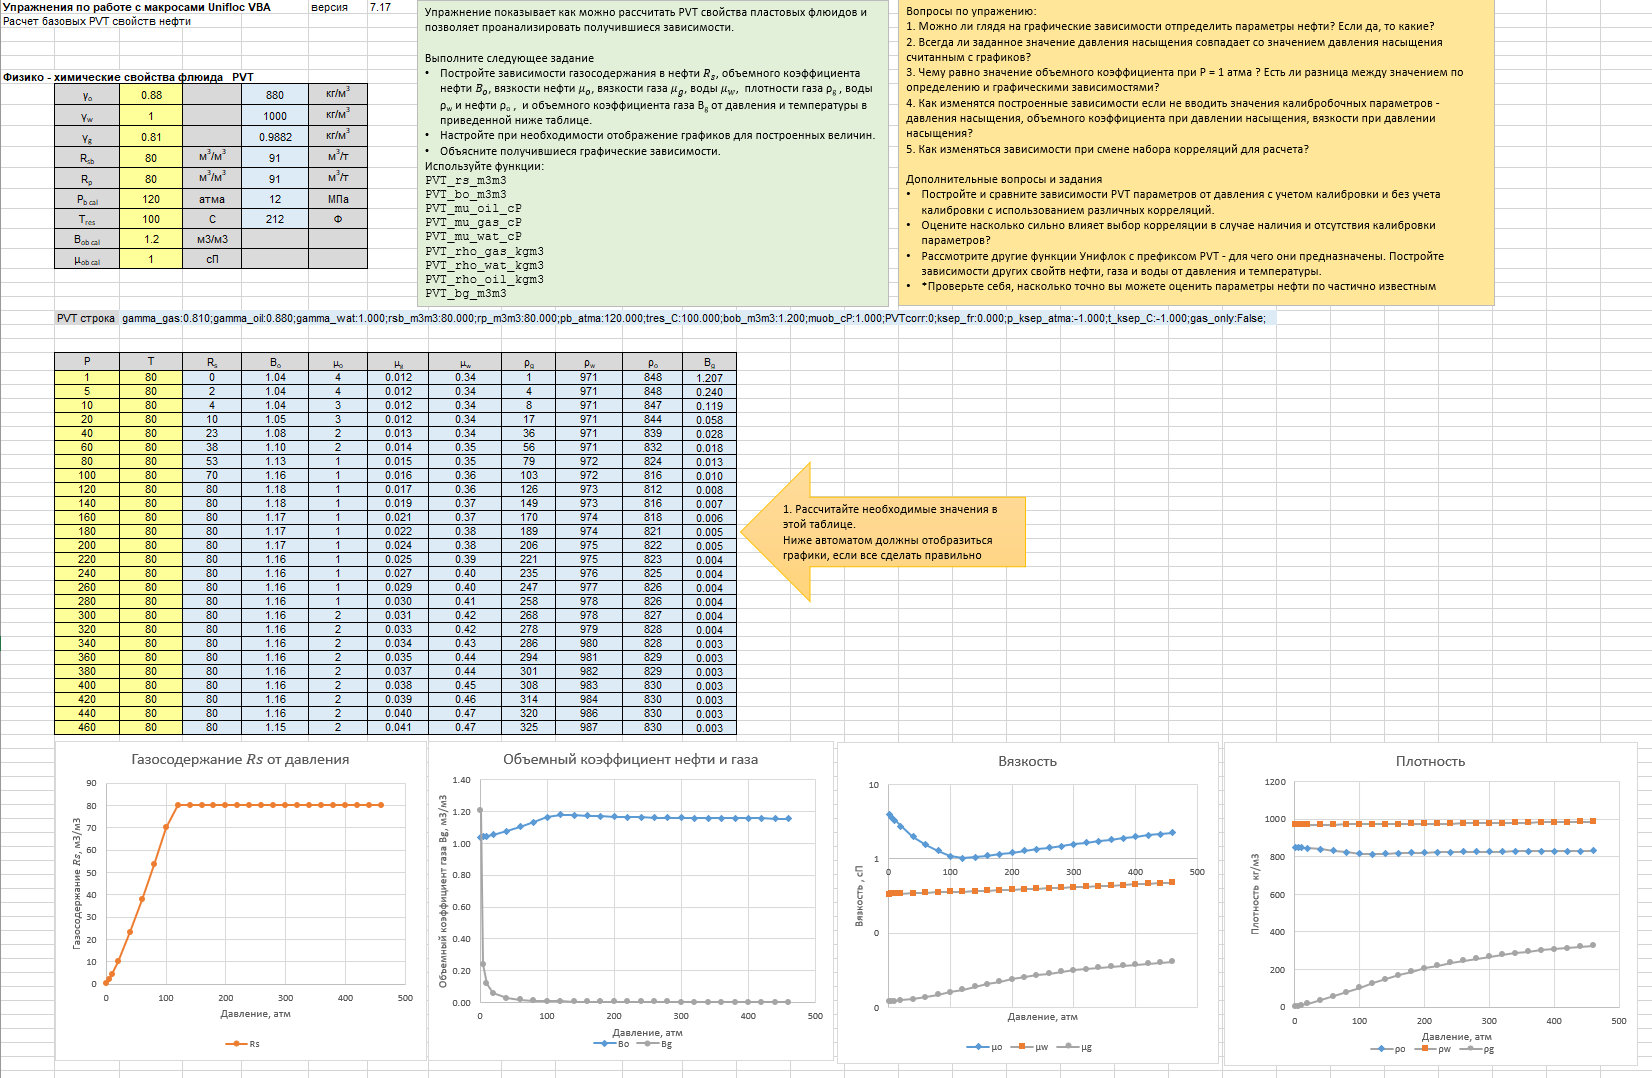
\includegraphics[width=1\linewidth]{Ex10_1}}
		\caption{Упражнение \texttt{ex010.PVT.xlsx} со всеми заполненными полями.}
		\label{ris:Ex10_1}
	\end{figure}
	
	\item Выполните задания указанные в описании. Задания просты -- требуется рассчитать таблицу значений для построения графиков и провести анализ построенных графиков. Названия необходимых функций указаны в описании  \ref{ris:Ex10_1}). Вопросы по упражнению помогут вам провести анализ. Текст заданий не приводится в описании, так как файлы упражнений первичны. Любые изменения скорее будут вноситься в файлы с заданиями, нежели в описание.
	
	\item Ответьте на вопросы по упражнению приведенные в рабочей книге.
	 
\end{enumerate}

\section{Расчет свойств потока флюидов}

PVT функции описывают свойства флюидов. Можно представить себе, что они описывают свойства флюидов находящихся в PVT бомбе - устройстве для отбора проб. В этом случае флюиды неподвижны и находятся в равновесном состоянии. На практике приходится иметь дело с флюидами двигающимися в скважине или трубопроводе - с потоком флюидов. В потоке флюидов добавляются дополнительные параметры -- расход флюидов или дебит $Q_{liq}, Q_g$ и обводненность $f_w$ -- показатель показывающий объемную долю воды в потоке. 
Функции работающие с потоками в \unf{} имеют префикс \mintinline{vb.net}{MF_}. Префикс должен намекать на многофазность потока и на самом деле плох с лингвистической точки зрения (multiphase - has no F letter), но удобен с программистской точки зрения и уже поздно его менять.

Файл примера \mintinline{vb.net}{ex011.Gas_fraction.xlsx} можно найти в папке \texttt{exercises} репозитория \unf{}.

\begin{enumerate}
	
	\item Откройте файл с упражнением \texttt{10.PVT.xlsx} (смотри рис. \ref{ris:Ex11_1}).
	
	\begin{figure}[h!]
		\center{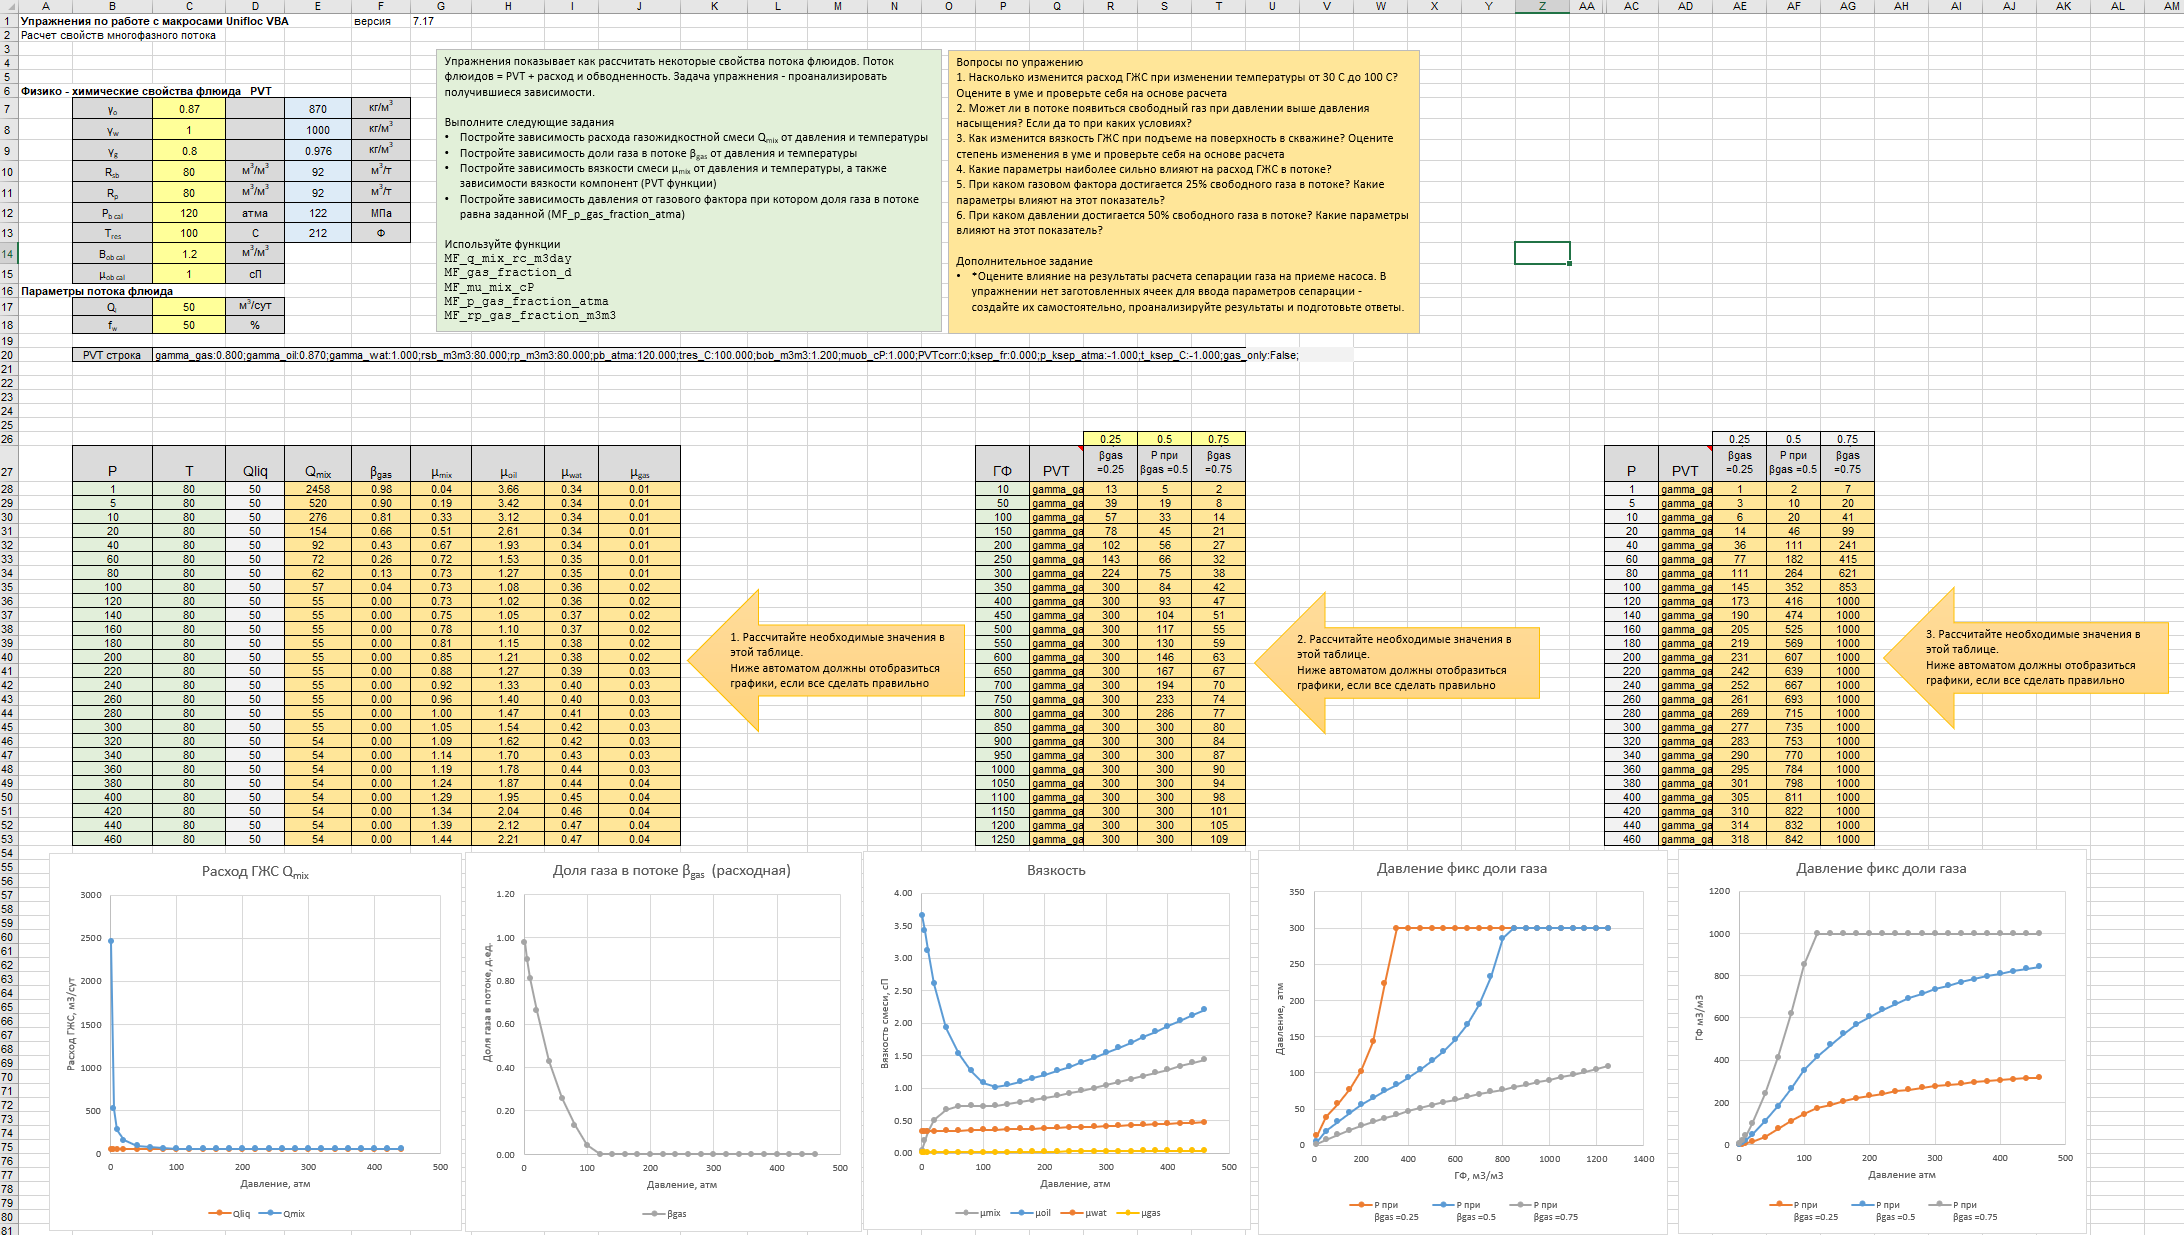
\includegraphics[width=1\linewidth]{Ex11_1}}
		\caption{Упражнение \mintinline{vb.net}{ex011.Gas_fraction.xlsx} со всеми заполненными полями }
		\label{ris:Ex11_1}
	\end{figure}
	
	\item Выполните задания указанные в описании. Задания просты -- требуется рассчитать три таблицы значений для построения графиков и провести анализ построенных графиков. Названия необходимых функций указаны в описании  \ref{ris:Ex11_1}). Вопросы по упражнению помогут вам провести анализ. Текст заданий не приводится в описании, так как файлы упражнений первичны. Любые изменения скорее будут вноситься в файлы с заданиями, нежели в описание.
	
	\item Ответьте на вопросы по упражнению приведенные в рабочей книге.
	
	\item Выполните дополнительное задание, если чувствуете силы. В дополнительном задании говорится о сепарации газа на приеме насоса. Имеется в виду следующее - если у нас есть пластовые флюиды, свойства которых мы знаем и можем задать, то после сепарации части свободного газа, что часто происходит на скважинном насосе, свойства флюида изменятся. Изменится его эффективное давление насыщения (потому что мы убрали часть газа) и газосодержание при давлении насыщения. И соответственно поплывут и остальные свойства. Это можно учесть задав в \mintinline{vb.net}{PVT_Encode()} три параметра - коэффициент сепарации газа $K_{sep}$, давление при которой произошла сепарации $P_{sep}$ и температуру при которой произошла сепарация $T_{sep}$. Подробнее про это можно найти в соответствующих разделах (поэтому тут это задание дополнительное).
	
\end{enumerate}

\section{Расчет производительности скважины}

Стационарная модель притока к скважине (закон Дарси с поправкой Вогеля) - одна из самых простых и распространенных моделей, широко применяемая в индустрии. \unf{} содержит функции позволяющие упростить расчет индикаторной кривой. Такие функции имеют префикс \mintinline{vb.net}{IPR_} от Inflow Performance Relationship.

Файл примера \mintinline{vb.net}{ex020.IPR.xlsx} можно найти в папке \texttt{exercises} репозитория \unf{}.

\begin{enumerate}
	
	\item Откройте файл с упражнением \texttt{ex020.IPR.xlsx} (смотри рис. \ref{ris:Ex20_1}).
	
		\begin{figure}[h!]
			\center{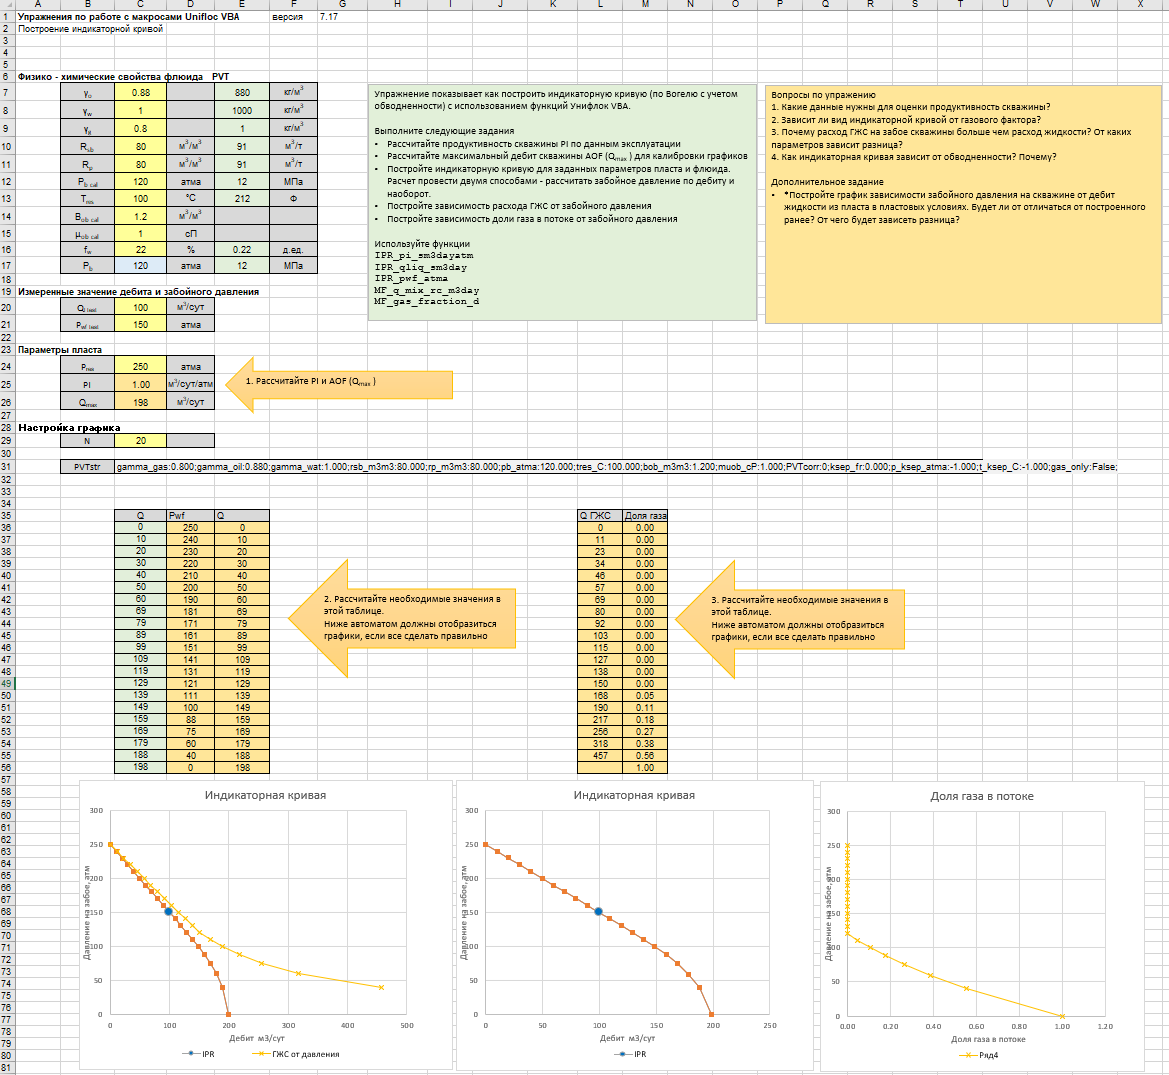
\includegraphics[width=1\linewidth]{Ex20_1}}
			\caption{Упражнение \mintinline{vb.net}{ex020.IPR.xlsx} со всеми заполненными полями }
			\label{ris:Ex20_1}
		\end{figure}

	\item Выполните задания указанные в описании. Задания просты -- требуется рассчитать три таблицы значений для построения графиков и провести анализ построенных графиков. Названия необходимых функций указаны в описании  \ref{ris:Ex11_1}). Вопросы по упражнению помогут вам провести анализ. Текст заданий не приводится в описании, так как файлы упражнений первичны. Любые изменения скорее будут вноситься в файлы с заданиями, нежели в описание.
	
	\item Ответьте на вопросы по упражнению приведенные в рабочей книге.
	
	\item Выполните дополнительное задание, если чувствуете силы.

\end{enumerate}

Коэффициент продуктивности $PI$ скважины рассчитывается в ячейке С25 по замеренным данным  с помощью функции

{ \small  \texttt{=IPR\_PI\_sm3dayatm(qltest\_;Pwftest\_;Pres\_;fw\_;Pb\_)}}

А максимальный дебит $Q_{max}$ при максимальной депрессии с забойным давлением равным нулю

{ \small  \texttt{=IPR\_Qliq\_sm3Day(PI\_;Pres\_;0;fw\_;Pb\_)}}




\section{Расчет штуцера}

Для контроля дебита и/или давления на добывающих скважинах вблизи устья может устанавливаться штуцер. Для штуцера, как для любого гидравлического элемента, возможно 4 варианта расчета - расчет давления по потоку, расчет давления против потока, расчет потока по давлениям и настройка модели штуцера по известным давлениям и потоку. В упражнении демонстрируются все варианты расчета. 

Файл примера \mintinline{vb.net}{ex040.MF_choke.xlsx} можно найти в папке \texttt{exercises} репозитория \unf{}.

\begin{enumerate}
	
	\item Откройте файл с упражнением \mintinline{vb.net}{ex040.MF_choke.xlsx} (смотри рис.\ref{ris:Ex40_1}).
	
	\begin{figure}[h!]
		\center{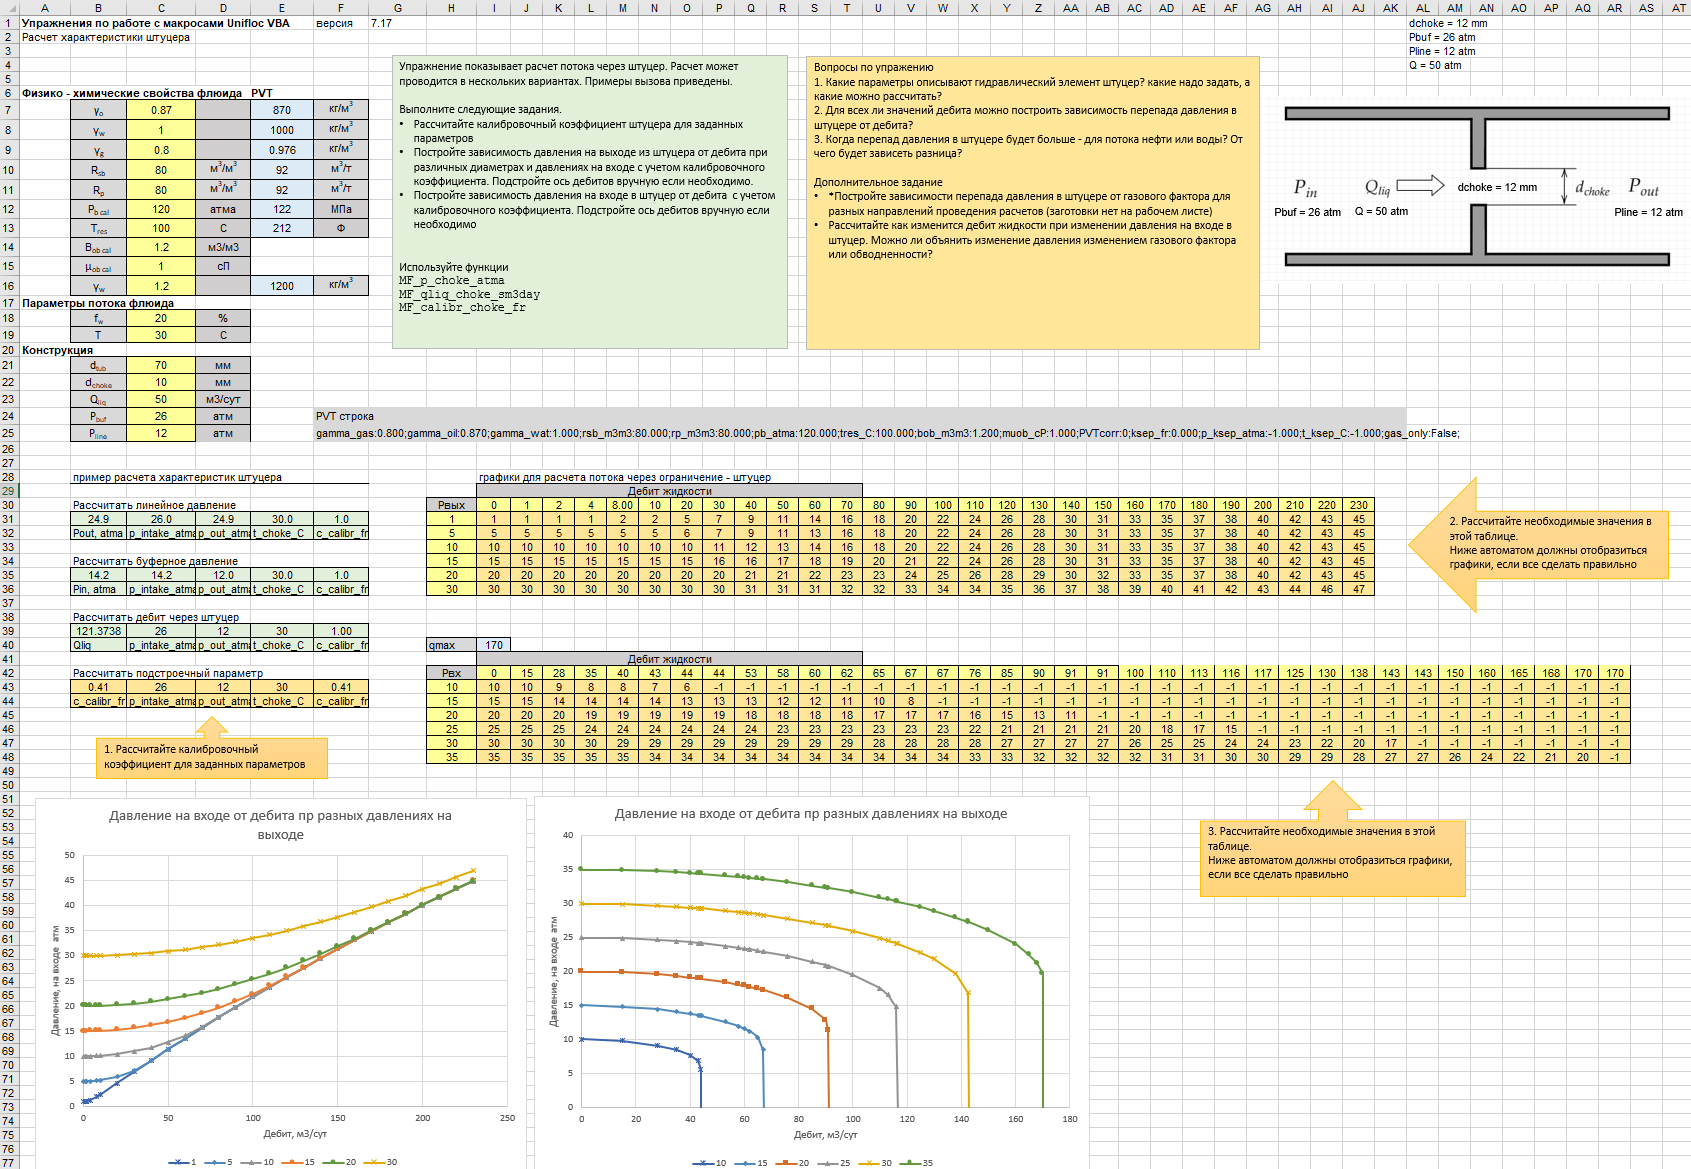
\includegraphics[width=1\linewidth]{Ex40_1}}
		\caption{Упражнение \mintinline{vb.net}{ex040.MF_choke.xlsx} со всеми заполненными полями }
		\label{ris:Ex40_1}
	\end{figure}
	
	\item Выполните задания указанные в описании. Названия необходимых функций указаны в описании  \ref{ris:Ex11_1}). При построении графиков может потребоваться изменить значения дебитов по которым проводится расчет для корректного отображения графиков. Текст заданий не приводится в описании, так как файлы упражнений первичны. Любые изменения скорее будут вноситься в файлы с заданиями, нежели в описание. 
	
	\item Ответьте на вопросы по упражнению приведенные в рабочей книге.
	
	\item Выполните дополнительное задание, если чувствуете силы.
	
\end{enumerate}


\section{Расчет распределения давления в трубе}
Расчет многофазных потоков в трубе - ключевой для анализа работы скважин и скважинного оборудования. Под расчетов трубы подразумевается в первую очередь расчет распределения давления. Иногда требуется рассчитать и распределение температуры. 
На распределение давления в трубе среди прочих параметров влияют режим потока газожидкостной смеси и явление проскальзывание газа. Недоучет данных параметров может привести к значительным ошибкам. Методы для расчета распределения давления можно разделить на две категории: корреляции, полученные экспериментальным путем и механистические модели, в основе которых заложены физические модели.

В \unf{} есть два набора функций для работы с трубой - простые по работе с прямым участком трубы \mintinline{vb.net}{MF_p_pipe} и более сложные по работе с участком трубопровода с учетом рельефа или инклинометрии \mintinline{vb.net}{MF_p_pipeline}

\subsection{Расчет прямолинейного участка трубы. Простой вариант}
Файл примера \mintinline{vb.net}{ex050.MF_pipe.xlsx} можно найти в папке \texttt{exercises} репозитория \unf{}.

\begin{enumerate}
	
	\item Откройте файл с упражнением \mintinline{vb.net}{ex050.MF_pipe.xlsx} (смотри рис.\ref{ris:Ex50_1}).
	
	\begin{figure}[h!]
		\center{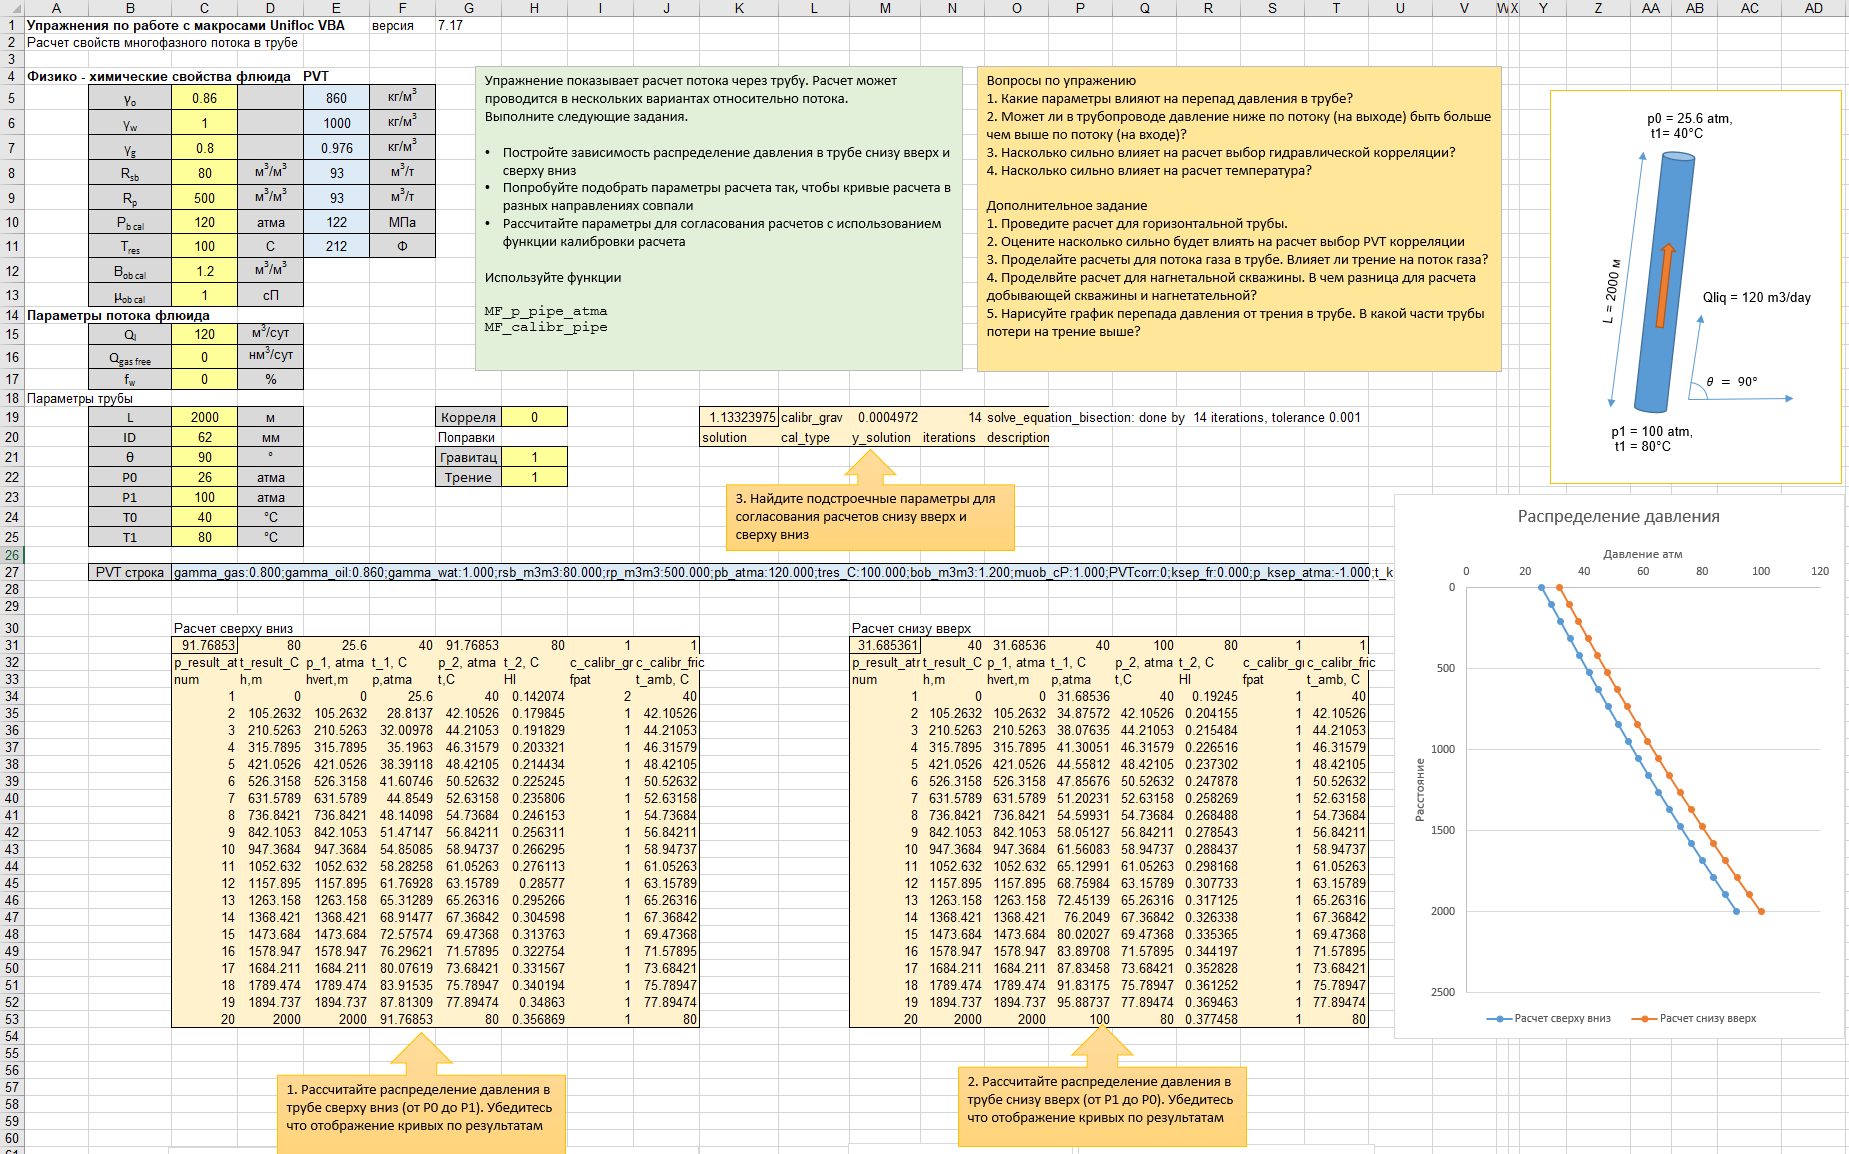
\includegraphics[width=1\linewidth]{Ex50_1}}
		\caption{Упражнение \mintinline{vb.net}{ex050.MF_pipe.xlsx} со всеми заполненными полями }
		\label{ris:Ex50_1}
	\end{figure}
	
	\item Выполните задания указанные в описании. Названия необходимых функций указаны в описании  \ref{ris:Ex50_1}). Текст заданий не приводится в описании, так как файлы упражнений первичны. Любые изменения скорее будут вноситься в файлы с заданиями, нежели в описание. 
	
	\item Ответьте на вопросы по упражнению приведенные в рабочей книге.
	
	\item Выполните дополнительное задание, если чувствуете силы.
	
\end{enumerate}





\section{Расчет коэффициентов сепарации}

Процессы сепарации на приеме погружного оборудования значительно влияют на процесс добычи. Как при естественной, так и при искусственной сепарации (при применении газосепараторов) меняются свойства многофазного потока, уменьшается газлифтный эффект, изменяется режим работы центробежного насоса.

В данном упражнении помимо стандартного определения PVT свойств требуется задать термобарические условия на приеме погружного оборудования (в месте, где происходит сепарация) и конструктивные параметры


\begin{figure}[h!]
	\center{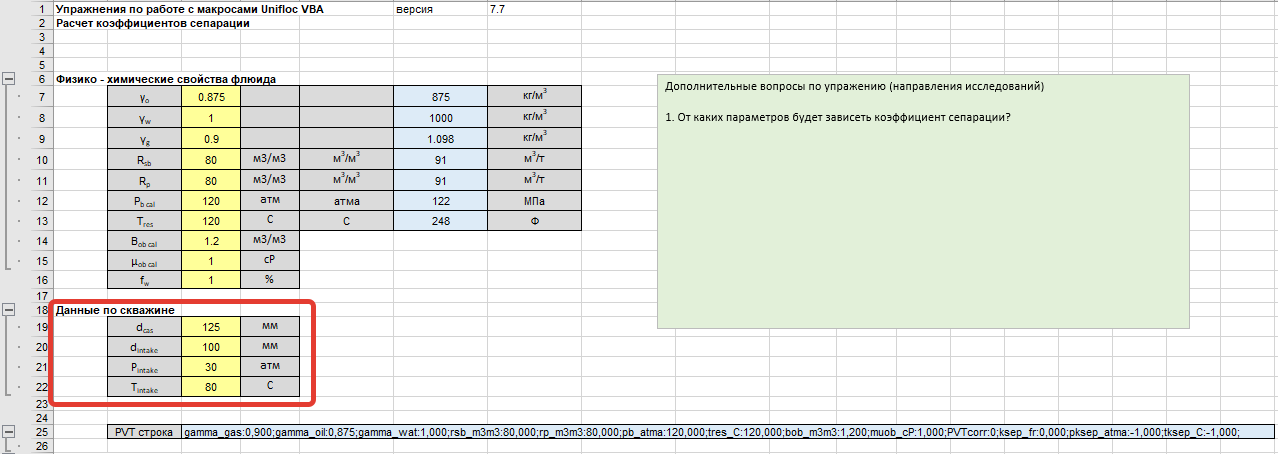
\includegraphics[width=1\linewidth]{Ex60_1}}
	\caption{Исходные данные для сепарации}
	\label{ris:Ex60_1}
\end{figure}

где

$d_{cas}$ - диаметр обсадной колонны, мм

$d_{intake}$ - диаметр приема погружного оборудования, мм

$P_{intake}$ - давление на приеме, атм

$T_{intake}$ - температура на приеме, С

Для вычисления коэффициента естественной сепарации в зависимости от дебита вставьте в ячейку E32 следующую формулу 

{ \small  \texttt{=MF\_ksep\_natural\_d(C32; wc\_; Pintake\_; Tintake\_; Dintake\_; Dcas\_; PVT\_str\_)}}

Для проведения экспериментов по влиянию изменения диаметра обсадной колонны воспользуйтесь в ячейке F32 формулой

{ \small  \texttt{=MF\_ksep\_natural\_d(C32; wc\_; Pintake\_; Tintake\_; Dintake\_; Dcas\_*cf\_dcas\_; PVT\_str\_)}}

При этом в ячейке F30 с помощью коэффициента Вы можете варьировать диаметр обсадной колонны

Для расчета доли газа в газосепараторе применяется функция

{ \small  \texttt{=MF\_gas\_fraction\_d(Pintake\_;Tintake\_;0;PVT\_str\_)*(1-F32)
}}

Коэффициент сепарации газосепаратора

{ \small  \texttt{=MF\_ksep\_gasseparator\_d(gassep\_type;G32;C32)
}}

При этом можно менять тип газосепаратора в ячейке H30

Общий коэффициент сепарации

{ \small  \texttt{=MF\_ksep\_total\_d(E32;H32)
}}

\begin{figure}[h!]
	\center{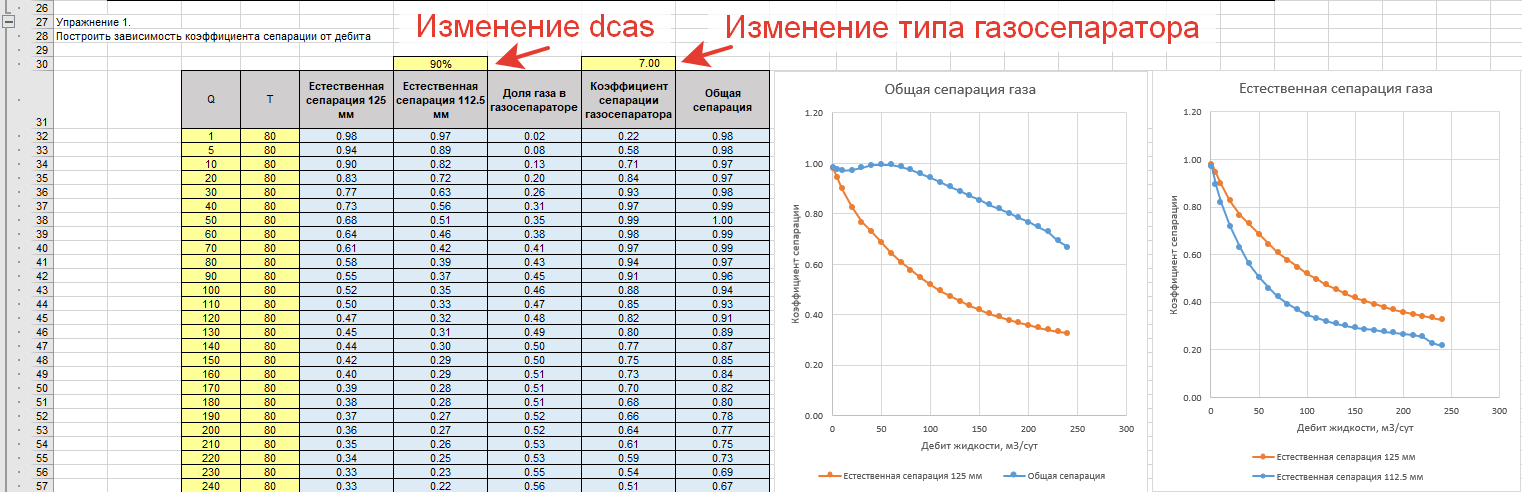
\includegraphics[width=1\linewidth]{Ex60_2}}
	\caption{Результаты расчета естественной и искусственной сепарации}
	\label{ris:Ex60_2}
\end{figure}

Вопросы к упражнению

\begin{enumerate}
	\item От каких параметров будет зависеть коэффициент сепарации?
	\item Как взаимосвязана естественная и искусственная сепарация? 
\end{enumerate}


\section{Анализ работы ЭЦН}

Сегодня доминирующая доля нефти в РФ добывается при помощи ЭЦН. Требуется детальное понимание основных особенностях эксплуатации данного оборудования, режимах работы, возможных осложнениях по причине высокой вязкости продукции, газосодержания, механических примесей и т.д.

Наиболее ценную информацию о работе насоса может дать его характеристика: зависимость параметров работы ЭЦН - напора, потребляемой мощности, перепада давления, КПД, от подачи (дебита скважины)

Для анализа работы скважины, оснащенной УЭЦН, требуются следующие исходные данные

\begin{enumerate}
	\item Физико - химические свойства флюида
	\item Данные по скважине
	\item Данные по ЭЦН
	\item Параметры пласта
\end{enumerate}

PVT свойства задаются аналогично предыдущим упражнениям, а для параметров, характеризующих скважину, приняты следующие обозначения

$H_{mes}$ - глубина скважины измеренная (вдоль ствола скважины), м

$H_{mes}- H_{vert}$ - удлинение ствола скважины, м

$H_{pump}$ - глубина спуска насоса, м

$ID_{cas}$ - внутренний диаметр обсадной колонны, мм

$OD_{tub}$ - внешний диаметр НКТ, мм

$ID_{tub}$ - внутренний диаметр НКТ, мм

$D_{intake}$ - диаметр приемной сетки ЭЦН, мм

$P_{buf}$ - буферное давление, атм

$P_{intake}$ - давление на приеме ЭЦН, атм

$T_{intake}$ - температура на приеме ЭЦН, С

$P_{dis}$ - давление на выкиде ЭЦН, атм

$P_{wf}$ - давление на забое, атм

$Q_{liq}$ - дебит жидкости в поверхностных условиях, м3/сут

$f_w$ - обводненность в поверхностных условиях, \%

\begin{figure}[h!]
	\center{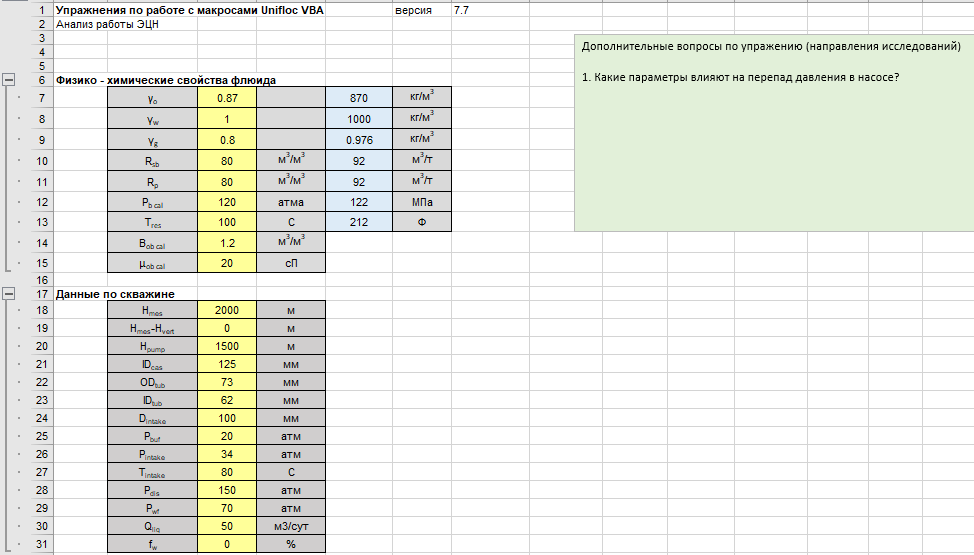
\includegraphics[width=1\linewidth]{Ex70_1}}
	\caption{Исходные данные для свойств флюида и параметров скважины}
	\label{ris:Ex70_1}
\end{figure}

Параметры, описывающие ЭЦН: 

ЭЦН $Q_{nom}$ - номинальная подача ЭЦН, м3/сут

ЭЦН $H_{nom}$ - номинальная напом ЭЦН, м

$F$ - частота питающего тока двигателя, Гц

ЭЦН $ID$ - идентификационный номер насоса (по формуле, см. ниже), находящийся в базе \unf

ЭЦН имя - обозначение насоса: название, габарит и номинальная подача (по формуле, см. ниже)

ЭЦН $Q_{max}$ - максимальная производительность насоса (по формуле, см. ниже), м3/сут

Ступени - количество ступеней, исходя из общего напора ЭЦН и напора одной ступени (по формуле, см. ниже), шт

$K_{sep_ГС}$ - коэффициент сепарации газосепаратора, \%

$P_{sep}$ - давление сепарации, атм

$T_{sep}$ - температура сепарации, С

Данные о пласте:

$P_{res}$ - пластовое давление, атм

$PI$ - коэффициент продуктивности скважины (по формуле, см. выше в упражнении IPR), м3/сут/атм

$\frac{dT}{dL}$ - геотермический градиент, град / 100 м

\begin{figure}[h!]
	\center{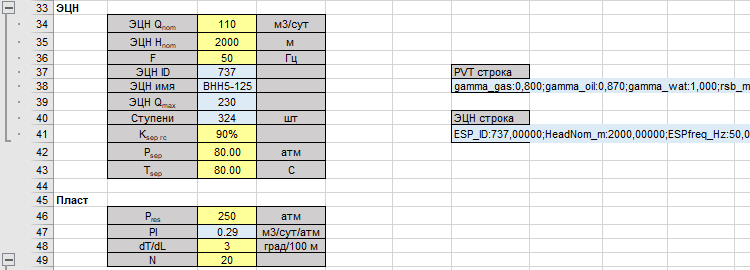
\includegraphics[width=1\linewidth]{Ex70_2}}
	\caption{Исходные данные для ЭЦН и пласта}
	\label{ris:Ex70_2}
\end{figure}

Для получения идентификационного номера насоса в базе \unf \ была использована формула

{ \small  \texttt{=ESP\_id\_by\_rate(Q\_ESP\_)}}

Для определения обозначения ЭЦН

{ \small  \texttt{=ESP\_name(C37)}}

Расчет максимально возможного дебита

{ \small  \texttt{=esp\_max\_rate\_m3day(Freq\_;PumpID\_)*1}}

Количество ступеней

{ \small  \texttt{=ЦЕЛОЕ(Head\_ESP\_/ESP\_head\_m(Q\_ESP\_;1;;PumpID\_))
}}

Также для удобства использования параметры насоса: ID, напор и рабочая частота, зашифровываются в строку с помощью функции

{ \small  \texttt{=ESP\_Encode\_string(PumpID\_;Head\_ESP\_;Freq\_)}}

Свободный газ негативно влияет на работу ЭЦН. В ячейке D51 вычисляется объемная доля газа на приеме газосепаратора с помощью формулы

{ \small  \texttt{=MF\_gas\_fraction\_d(Pintake\_;Tintake\_;fw\_;PVTstr)}}
 
В соседней ячейке D50 для удобного расположения задается вязкость в сПуаз

Построение напорной характеристики данного насоса выполняется с учетом вязкости перекачиваемой продукции. Реализованный метод пересчета характеристики с воды на вязкую жидкость Института Гидравлики позволяет учитывать изменение рабочих параметров из-за данного негативного влияния.

Для вычисления напора в метрах водного столба в ячейке D54 воспользуйтесь формулой

{ \small  \texttt{=ESP\_head\_m(C54;NumStage\_;Freq\_;PumpID\_;mu)}}

КПД ЭЦН в долях единиц 

{ \small  \texttt{=ESP\_eff\_fr(C54;NumStage\_;Freq\_;PumpID\_;mu)}}

Потребляемую ЭЦН мощность в Вт

{ \small  \texttt{=ESP\_Power\_W(C54;NumStage\_;Freq\_;PumpID\_;mu)}}

\begin{figure}[h!]
	\center{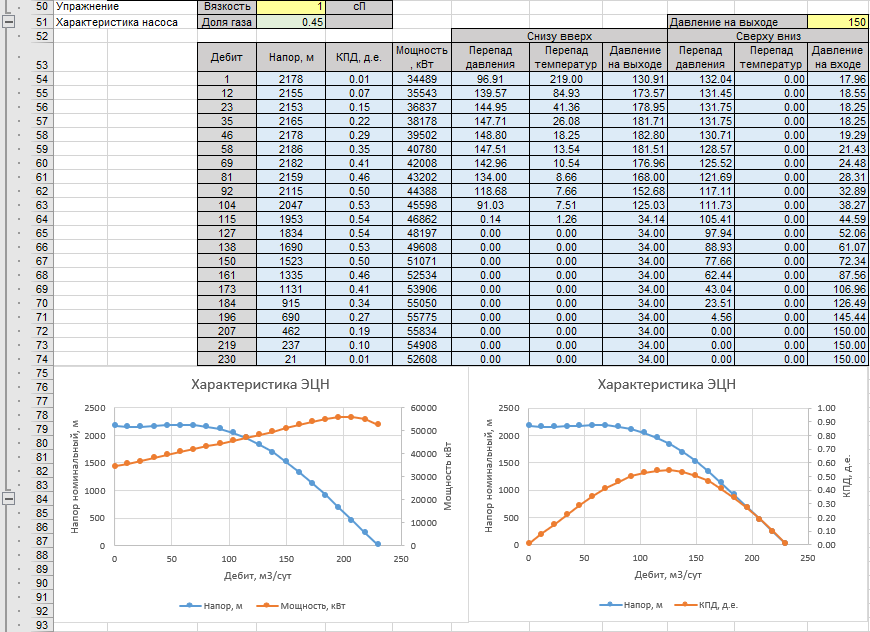
\includegraphics[width=1\linewidth]{Ex70_3}}
	\caption{Напорные характеристики ЭЦН с поправкой на вязкость}
	\label{ris:Ex70_3}
\end{figure}

Расчет перепада давления, развиваемого насосом, может происходить методом "сверху-вниз" \  и "снизу-вверх" \ , при этом расчет перепада температур только методом "снизу-вверх". Функция расчета перепада давления и температуры возвращает массив значений, т.е. одновременно перепад давления и температуры. Кроме того, входным параметром для данной функции является направление расчета. Для вычисления выделите диапазон G54:H54, наберите формулу

{ \small  \texttt{=ESP\_dP\_atm(C54; fw\_; Pintake\_; NumStage\_; Freq\_; PumpID\_; PVTstr; Tintake\_; 0)}}

и после нажмите сочетание клавиш  Ctrl+Shift+Enter. Далее протяните результат до полного заполнения двух столбцов.

Зная давление на приеме и перепад давления в ЭЦН, давление на выходе ЭЦН можно легко посчитать по формуле

{ \small  \texttt{=G54+Pintake\_}}

Предварительно задав давление на выходе ЭЦН в ячейке L51 возможно посчитать перепад давления методом "сверху-вниз"\ аналогичным образом по формуле

{ \small  \texttt{=ESP\_dP\_atm(C54; fw\_; Pdis\_; NumStage\_; Freq\_; PumpID\_; PVTstr; Tintake\_; Tintake\_; 0)}}

И давление на входе, зная давление на выходе и перепад давления

{ \small  \texttt{=Pdis-J54}}

\begin{figure}[h!]
	\center{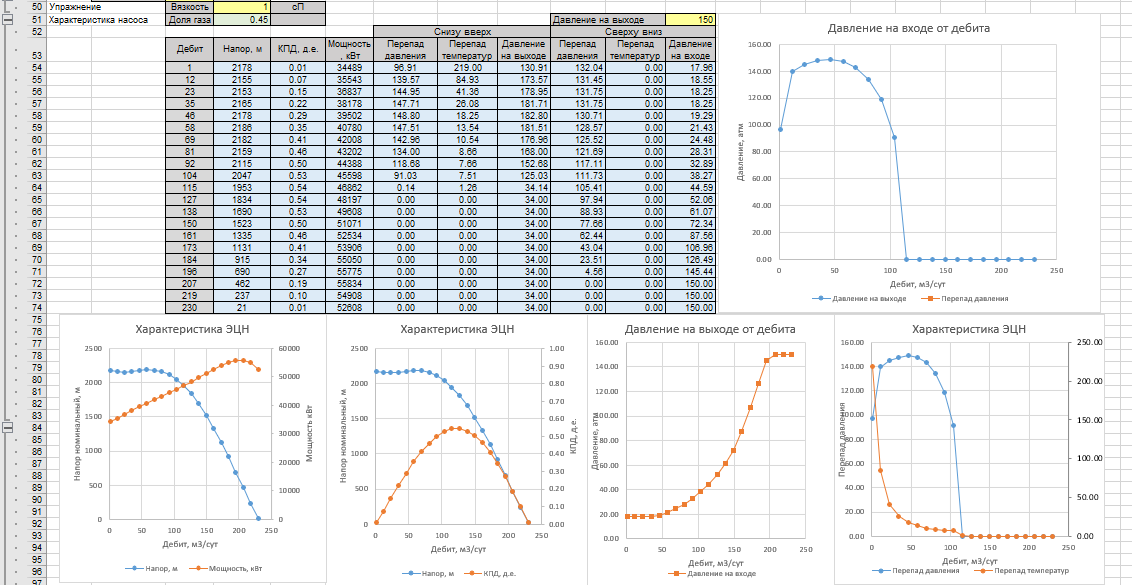
\includegraphics[width=1\linewidth]{Ex70_4}}
	\caption{Расчет перепада давления и температур в ЭЦН в зависимости от дебита}
	\label{ris:Ex70_4}
\end{figure}

Вопросы для упражнения:

\begin{enumerate}
	\item Какие параметры влияют на перепад давления в насосе?
	\item Насколько сильно влияет вязкость на напорные характерситики ЭЦН?
	\item Как влияет на работу ЭЦН изменение частоты?
\end{enumerate}


\section{Анализ работы ПЭД}

Упражнение показывает характеристики погружного асинхронного электрического двигателя, применяемого в УЭЦН.

Также стоит отметить, что расчетные функции предназначаются для образовательных целей. Детального сопоставления расчетных характеристик с фактическими не проводилось. (06.2019)

Для выполнения упражнения необходимо задать параметры электродвигателя

$U_{nom}$ - номинальное напряжение ПЭД, В

$F_{nom}$ - номинальная частота тока, Гц

$I_{nom}$ - номинальная сила тока, А

$ID$ - способ инициализации данных двигателя. 1 - по фактическим значениям параметров (по паспорту), 2 - по схеме замещения Гридина

А также рабочее напряжение $U$, В и рабочую частоту тока $F$, Гц

После этого в ячейке С10 будет произведен расчет номинальной мощности ПЭД с помощью функции

{ \small  \texttt{=Motor\_Pnom\_kW(Unom;Inom;Fnom;ID)}}

\begin{figure}[h!]
	\center{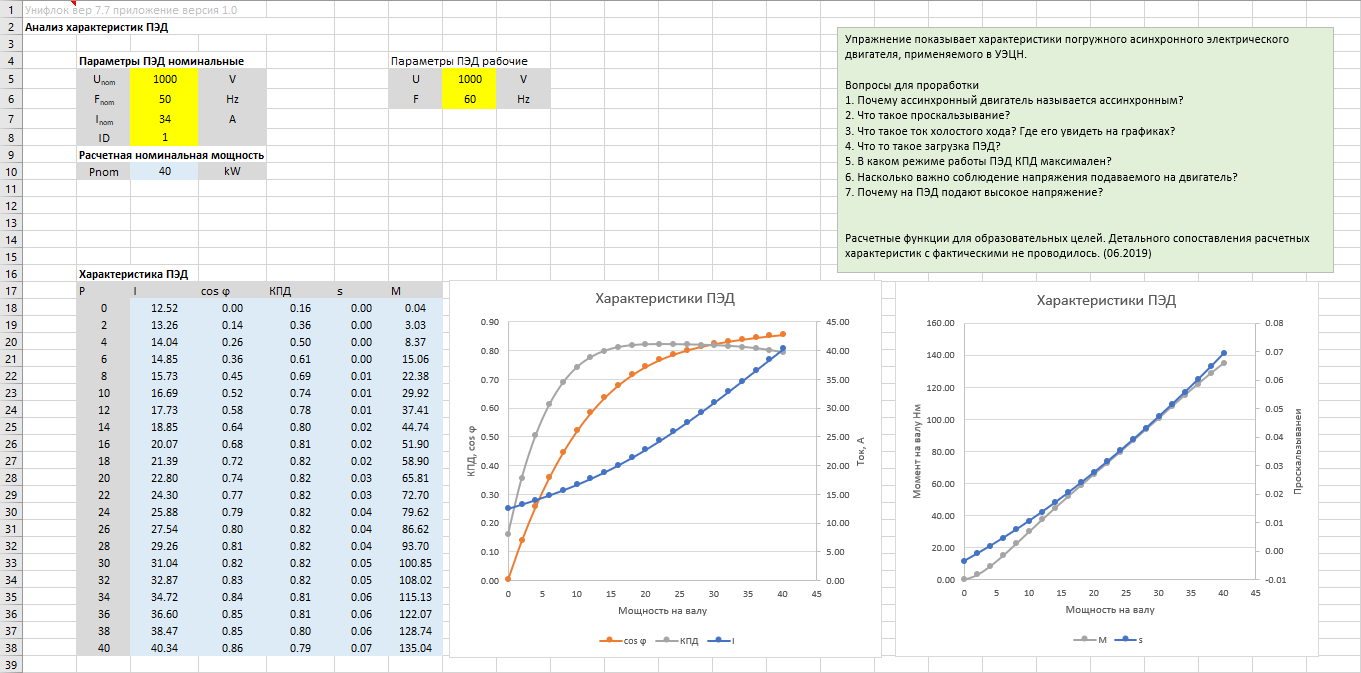
\includegraphics[width=1\linewidth]{Ex80_1}}
	\caption{Исходные данные ПЭД и различные характеристики в зависимости от мощности на валу}
	\label{ris:Ex80_1}
\end{figure}

Для построения характеристики ПЭД (параметры двигателя от мощности на валу $M$) воспользуйтесь следующими формулами

Определение тока двигателя $I$, A

{ \small  \texttt{=motor\_I\_A(B18;F;U;Unom;Inom;Fnom;ID)}}

Расчет $cos \varphi $

{ \small  \texttt{=motor\_CosPhi\_d(B18;F;U;Unom;Inom;Fnom;ID)}}

КПД, д.ед.

{ \small  \texttt{=motor\_Eff\_d(B18;F;U;Unom;Inom;Fnom;ID)}}

Проскальзывание $S$

{ \small  \texttt{=motor\_S\_d(B18;F;U;Unom;Inom;Fnom;ID)}}

Момент на валу $M$, Н*м

{ \small  \texttt{=motor\_M\_Nm(B18;F;U;Unom;Inom;Fnom;ID)}}

\begin{figure}[h!]
	\center{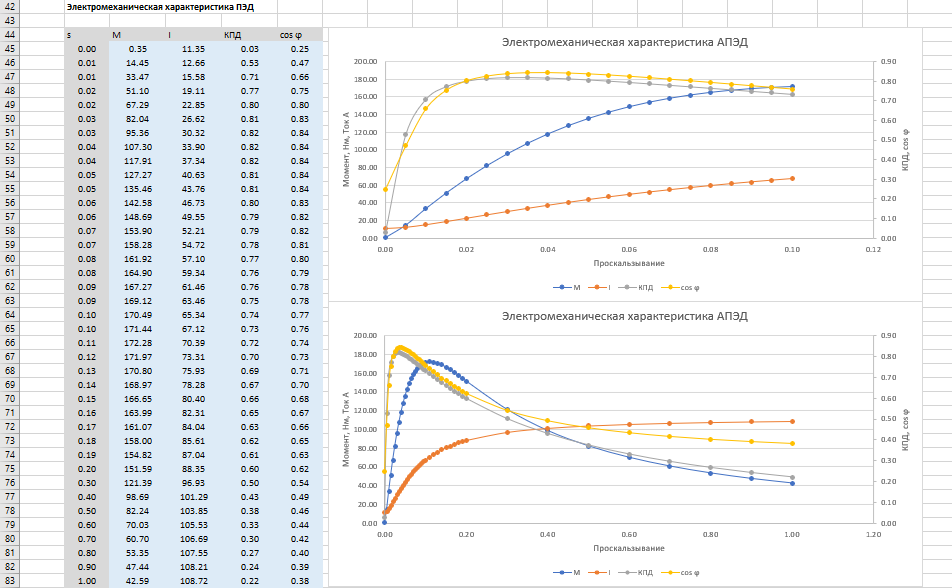
\includegraphics[width=1\linewidth]{Ex80_2}}
	\caption{Электромеханическая характеристика АПЭД}
	\label{ris:Ex80_2}
\end{figure}

Для расчета электромеханической характеристики АПЭД (параметры двигателя в зависимости от проскальзывания $S$) используйте формулы

Момент на валу $M$, Н*м 

{ \small  \texttt{=motor\_M\_slip\_Nm(B45;F;U;Unom;Inom;Fnom;0)}}

Сила тока $I$, А

{ \small  \texttt{=motor\_I\_slip\_A(B45;F;U;Unom;Inom;Fnom;0)}}

КПД, д.ед.

{ \small  \texttt{=motor\_Eff\_slip(B45;F;U;Unom;Inom;Fnom;0)}}

Расчет $cos \varphi $

{ \small  \texttt{=motor\_CosPhi\_slip(B45;F;U;Unom;Inom;Fnom;0)}}


\begin{figure}[h!]
	\center{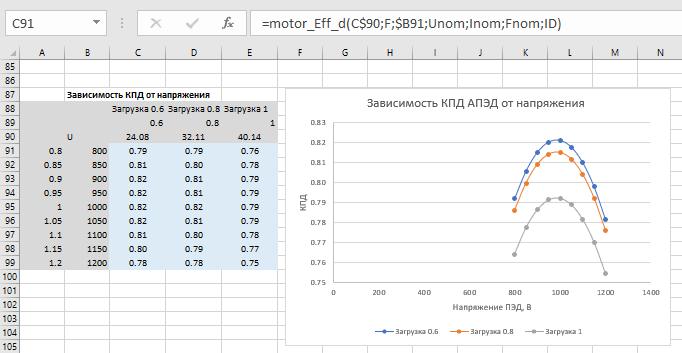
\includegraphics[width=1\linewidth]{Ex80_3}}
	\caption{Зависимость КПД АПЭД от напряжения и загрузки}
	\label{ris:Ex80_3}
\end{figure}

Для проведения исследований по напряжению ПЭД воспользуйтесь следующими формулами для значений загрузки двигателя 0.6, 0.8, 1 

{ \small  \texttt{=motor\_Eff\_d(C\$90;F;\$B91;Unom;Inom;Fnom;ID)}}

{ \small  \texttt{=motor\_Eff\_d(D\$90;F;\$B91;Unom;Inom;Fnom;ID)}}

{ \small  \texttt{=motor\_Eff\_d(E\$90;F;\$B91;Unom;Inom;Fnom;ID)}}

в ячейках C91, E91, D91 соответственно. "Протянув"\ значения Вы можете заполнить таблицу.

Вопросы для упражнения:

\begin{enumerate}
	\item Почему ассинхронный двигатель называется ассинхронным?
	\item Что такое проскальзывание?
	\item Что такое ток холостого хода? Где его увидеть на графиках?
	\item Что то такое загрузка ПЭД?
	\item В каком режиме работы ПЭД КПД максимален?
	\item Насколько важно соблюдение напряжения подаваемого на двигатель?
	\item Почему на ПЭД подают высокое напряжение?
\end{enumerate}


\section{Анализ работы фонтанирующей скважины}

При достаточном количестве естественной энергии скважина может фонтанировать. Инженерные расчеты требуются как для оптимизации работы самого подъемника, так и системы "скважина-пласт".

Для упражнения требуется задать PVT свойства флюидов, конструкцию скважины, свойства пласта и текущий режим работы скважины (дебит). Все исходные данные заполняются аналогично предыдущим упражнениям за исключением функции, объединяющей все данные о скважине в одну строку, расположенной в ячейке  $G23$

{ \small  \texttt{=well\_encode\_string(Hmes\_;Htube\_;Udl\_;Dcas\_;Dtub\_;0;;Twf\_;Tbuf\_)
}}

\begin{figure}[h!]
	\center{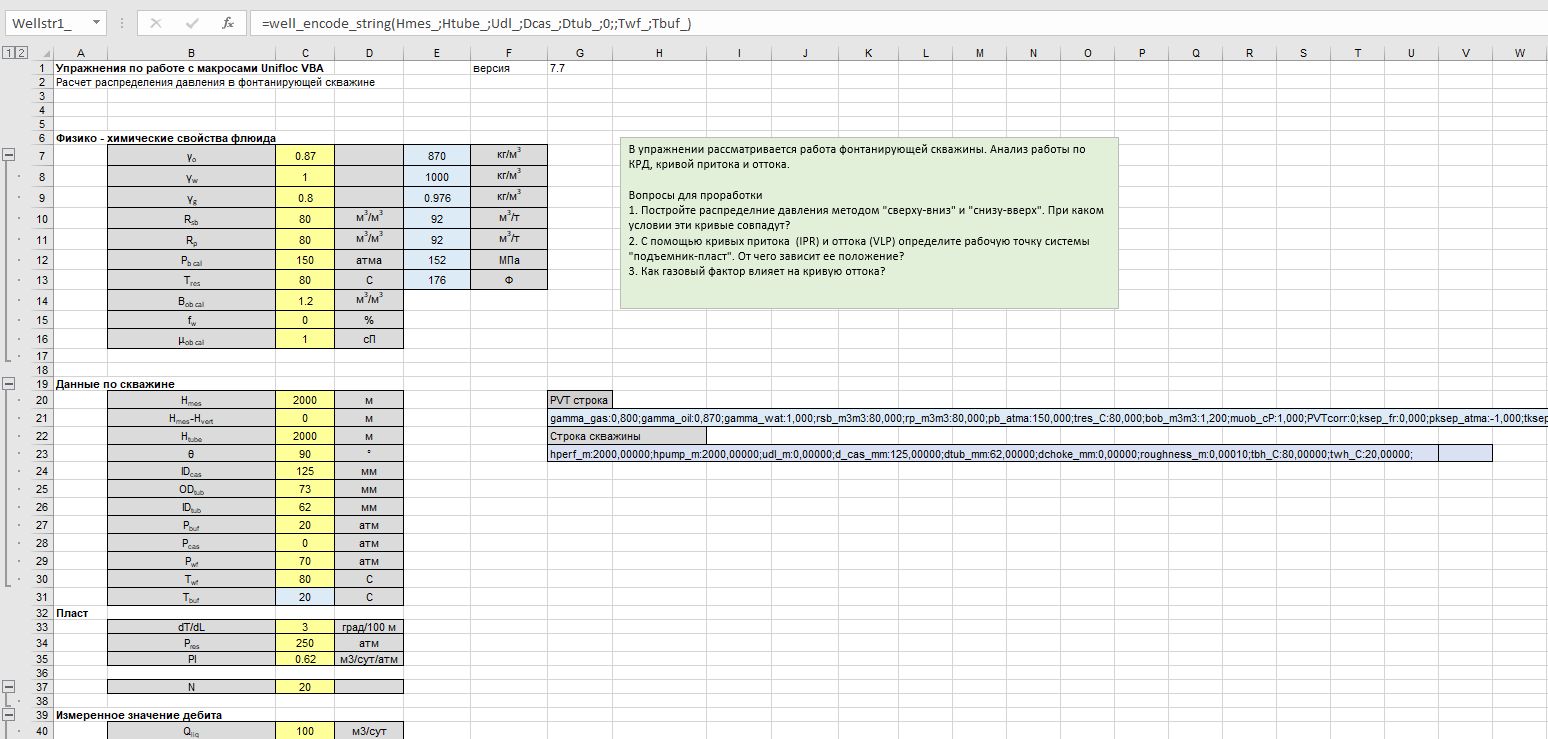
\includegraphics[width=1\linewidth]{Ex90_1}}
	\caption{Исходные данные для расчета фонтанирующей скважины}
	\label{ris:Ex90_1}
\end{figure}

В первой части задания требуется построить распределение давления в скважине методом сверху-вниз и снизу-вверх, задавая при этом граничные условия - давление на устье и на забое соответственно. Для расчета воспользуйтесь в ячейке $E50$ функцией

{ \small  \texttt{=MF\_p\_pipe\_atma(Qtest\_; fw\_;C49; C50;E49;PVRstr1\_; theta\_;Dtub\_;;D49;D50)
}}

"протянув"\ ее на весь столбец. Расчет снизу-вверх выполните аналогичным образом. Обратите внимание, что при правильных расчетах КРД должны совпадать - решение не должно зависеть от направления.

\begin{figure}[h!]
	\center{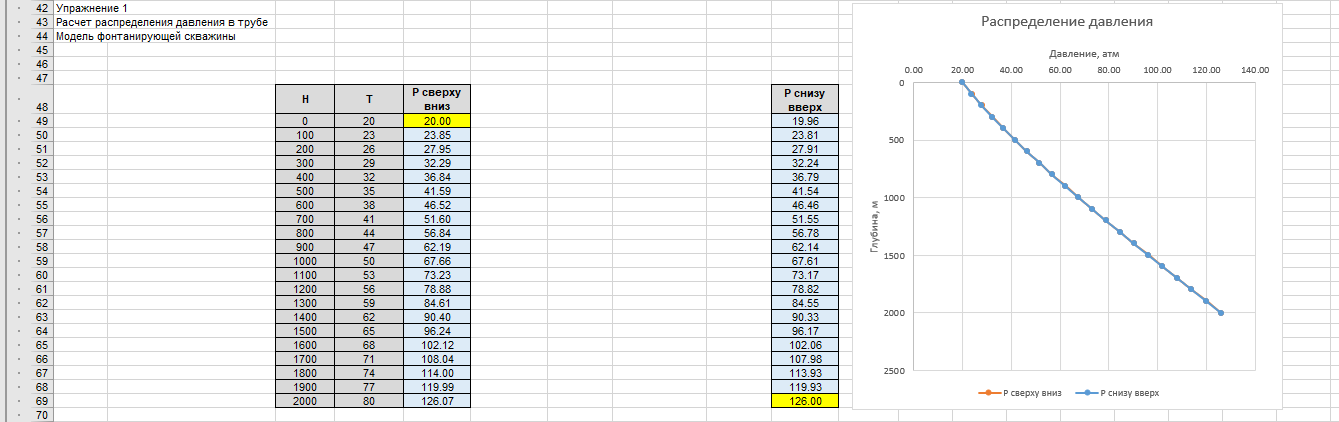
\includegraphics[width=1\linewidth]{Ex90_2}}
	\caption{Расчет КРД в фонтанирующей скважине}
	\label{ris:Ex90_2}
\end{figure}

Во второй части упражнения необходимо построить кривую притока (индикаторную кривую, по Вогелю) и кривую оттока (зависимость давления в начале подъемной трубы от дебита при неизменном давление на выходе). Забойное давление принимается равным рассчитанному из предыдущей части упражнения. Максимальный дебит скважины и коэффициент продуктивности можно варьировать вместе с обводненностью продукции скважины для анализа добывающей системы. Точка пересечения кривых притока и оттока будет являться рабочей точкой системы "пласт-скважина".

Для вычисления забойного давления для индикаторной кривой воспользуйтесь в ячейке $F78$ уже знакомой Вам функцией

{ \small  \texttt{=IPR\_Pwf\_atma(PI\_1;Pres\_;E78;fw\_;Pb\_)}}

Расчет забойного давления по устьевому в ячейке $G78$ примените функцию
 
{ \small  \texttt{=well\_pwf\_plin\_atma(E78;fw\_;Pbuf\_; Pcas\_; Wellstr1\_; PVRstr1\_; ;1;;;;;;1)}} 

Для другой величины обводненности продукции в $H78$ при анализе дальнейшей работы

{ \small  \texttt{=well\_pwf\_plin\_atma(E78;fw\_2;Pbuf\_; Pcas\_; Wellstr1\_; PVRstr1\_; ;1;;;;;;1)}} 

Заполнив таблицу до конца Вы получите следующий результат

\begin{figure}[h!]
	\center{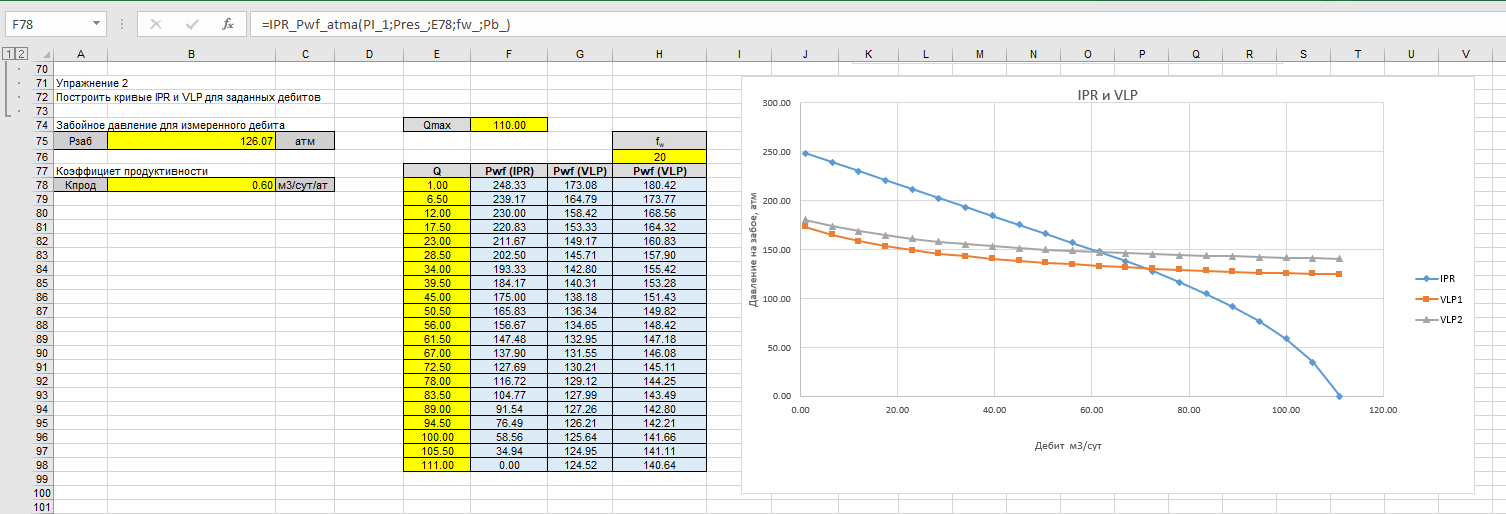
\includegraphics[width=1\linewidth]{Ex90_3}}
	\caption{Кривые оттока и притока для узлового анализа работы фонтанирующей скважины}
	\label{ris:Ex90_3}
\end{figure}

Для анализа влияния ГФ скважины на забойное давление воспользуйтесь теми же самыми функциями, за исключением того, что каждый раз будет меняться PVT строка свойств флюидов

В ячейке $H108$ 

{ \small  \texttt{=well\_pwf\_plin\_atma(Qtest\_;fw\_;Pbuf\_;Pcas\_;Wellstr1\_;G108;;1;;;;;;1)}}

В ячейке $I108$ 

{ \small  \texttt{=well\_pwf\_plin\_atma(Qtest\_;fw\_3;Pbuf\_;Pcas\_;Wellstr1\_;G108;;1;;;;;;1)}}

\begin{figure}[h!]
	\center{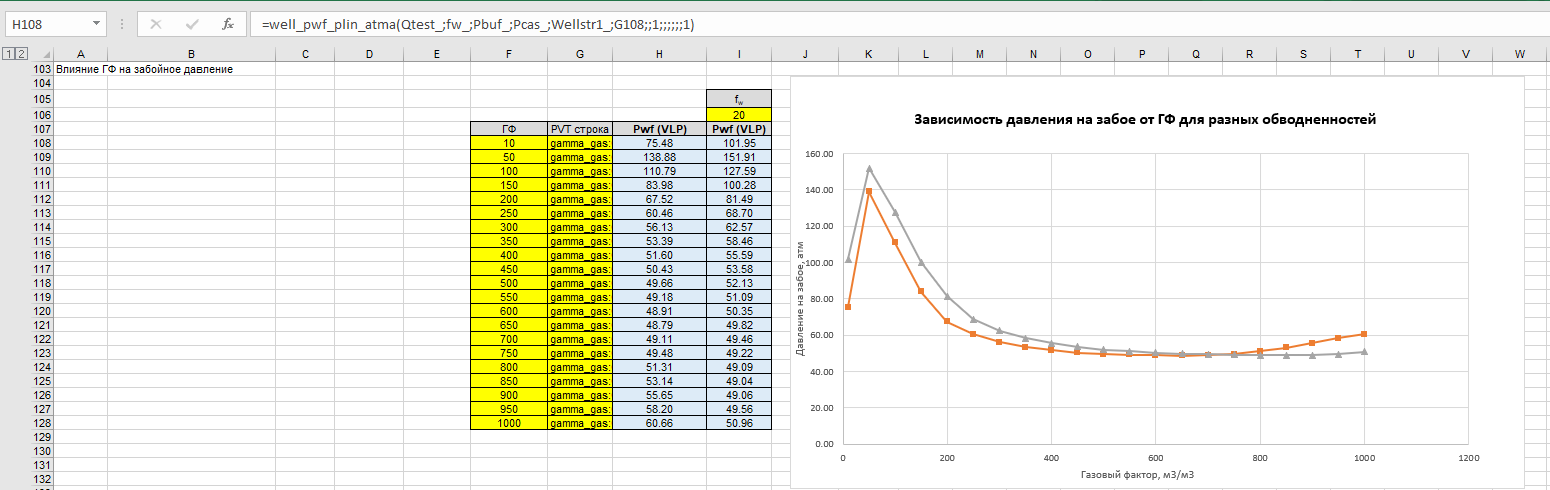
\includegraphics[width=1\linewidth]{Ex90_4}}
	\caption{Влияние газового фактора и обводненности на забойное давление}
	\label{ris:Ex90_4}
\end{figure}

Теперь Вы можете ответить на вопросы:

Вопросы для проработки

\begin{enumerate}
	\item Постройте распределние давления методом сверху-вниз и снизу-вверх. При каком условии эти кривые совпадут?
	\item С помощью кривых притока  (IPR) и оттока (VLP) определите рабочую точку системы "скважина-пласт". От чего зависит ее положение?
	\item Как газовый фактор влияет на кривую оттока?
\end{enumerate}

\section{Анализ работы скважины, оснащенной УЭЦН}

По сравнению с моделью фонтанирующей скважины в данный расчет добавляются такие важные элементы, как сепарация на приеме погружного оборудования и напорная характеристика ЭЦН. К стандартным исходным данным добавляется вторая PVT строка ($G45$) для разделения упражнения на 2 части. 

{ \small  \texttt{=PVT\_encode\_string(gamma\_gas\_; gamma\_oil\_; ; Rsb\_; Rp\_; Pb\_; Tres\_; Bob\_; mu\_;; KsepGasSep\_; PKsep2; TKsep2)
}}

Стоит сразу отметить важность определения давления и температуры, при которой происходит сепарация газа в затрубное пространство. При неизвестном давлении на приеме погружного оборудования (давлении сепарации) требуется определить его с помощью гидравлической корреляции, например, при расчете снизу-вверх от забойного давления. Однако расчет перепада давления в трубе зависит от PVT свойств, в том числе давления сепарации - поэтому требуется итеративный подход для изменения давления сепарации до тех пор, пока оно не окажется стабильным (и равным давлению на приеме погружного оборудования по гидравлической корреляции). Т.к. при сепарации происходит модификация флюида, пренебрежение согласованностью приведет к неправильному расчету - поток может быть дегазированным на забое или наоборот с высокой долей газа в насосе или НКТ. Изменять давление сепарации $P_{sep}$ можно в ячейке $C43$

\begin{figure}[h!]
	\center{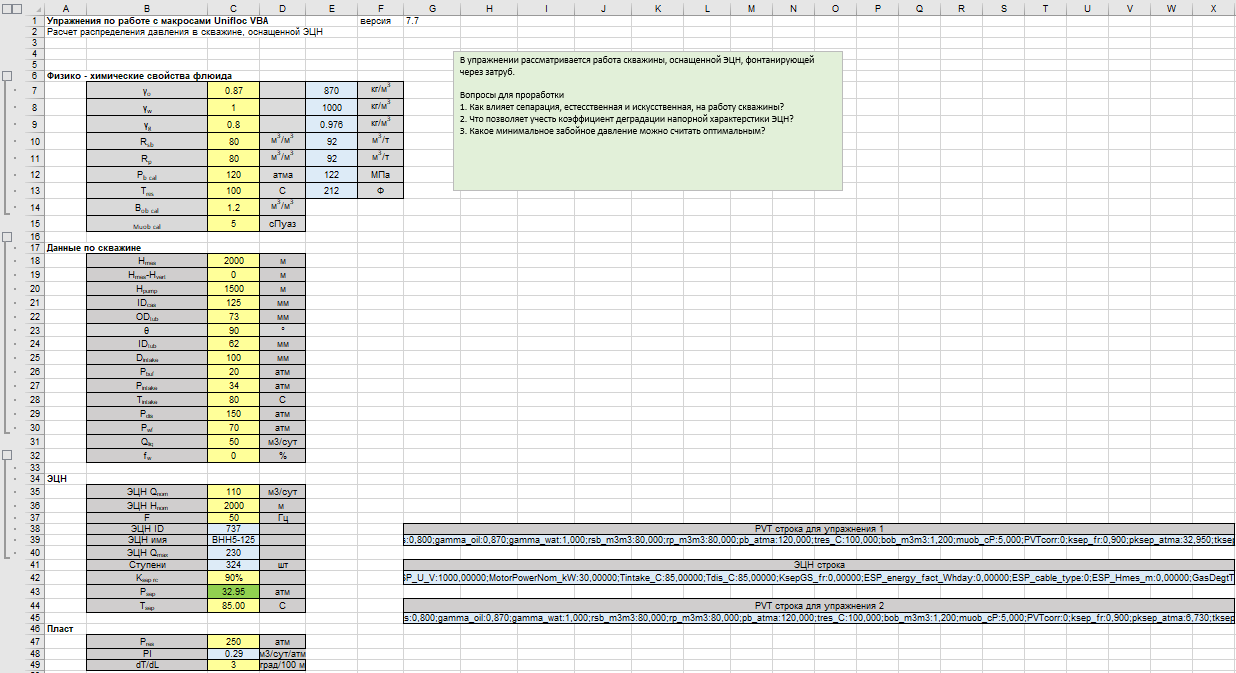
\includegraphics[width=1\linewidth]{Ex100_1}}
	\caption{Исходные данные для расчета скважины, оснащенной УЭЦН}
	\label{ris:Ex100_1}
\end{figure}

В первой части упражнения предлагается построить распределение давления в скважине с постоянным дебитом. 

Кривую давления от забоя до приема можно получить с помощью функции

{ \small  \texttt{=MF\_p\_pipe\_atma(Q\_;fw\_;C83;C82; F83;PVT\_str\_; theta\_; Dtub\_;; D83;D82)
}}

"протянув"\ ее до глубины спуска оборудования. С учетом сепарации, которая подробно описывалась выше, требуется изменять значение давления сепарации $P_{sep}$ в исходных данных ($C43$) пока оно не станет равным расчетному.

Затем в ячейке $G78$ можно определить коэффициент естественной сепарации

{ \small  \texttt{=MF\_ksep\_natural\_d(Q\_; wc\_; Pintake\_; Tintake\_; Dintake\_; Dcas\_; PVT\_str\_)
}}

А в $H78$ искусственную с помощью 

{ \small  \texttt{=MF\_ksep\_total\_d(G78;KsepGasSep\_)
}}

Распределение давления в НКТ рассчитывается методом сверху-вниз, начиная с ячейки $K64$

{ \small  \texttt{=MF\_p\_pipe\_atma(Q\_;fw\_;C63;C64;K63;PVT\_str\_;theta\_;Dintake\_;;D63;D64)
}}

Таким образом можно получить перепад давления в насосе не прибегая к расчету самого насоса - он будет равен разнице между давлением в нижней точке НКТ и на приеме погружного оборудования (ячейка $N78$). Но по напорной характеристике с помощью функции в $M78$

{ \small  \texttt{=ESP\_dP\_atm(Q\_; fw\_;Pintake\_; NumStage\_;Freq\_; PumpID\_; PVT\_str\_;Tintake\_; 0;1;;D60)
}}

также можно получить данное значение, воспользовавшись коэффициентом деградации напорной характеристики ЭЦН в $D60$ для адаптации модели. При совпадении результатов двух независимых расчетов возможно оценить состояние погружного оборудования.

Полезным для анализа работы добывающей системы будет знание о доли газа в потоке как до приема погружного оборудования (начиная с ячейки $I83$)

{ \small  \texttt{=MF\_gas\_fraction\_d(F83;D83;fw\_;PVT\_str\_)
}}

так и после сепарации в НКТ (с $J78$)

{ \small  \texttt{=MF\_gas\_fraction\_d(K78;D78;fw\_;PVT\_str\_)
}}

На этом первая часть упражнения завершается.

\begin{figure}[h!]
	\center{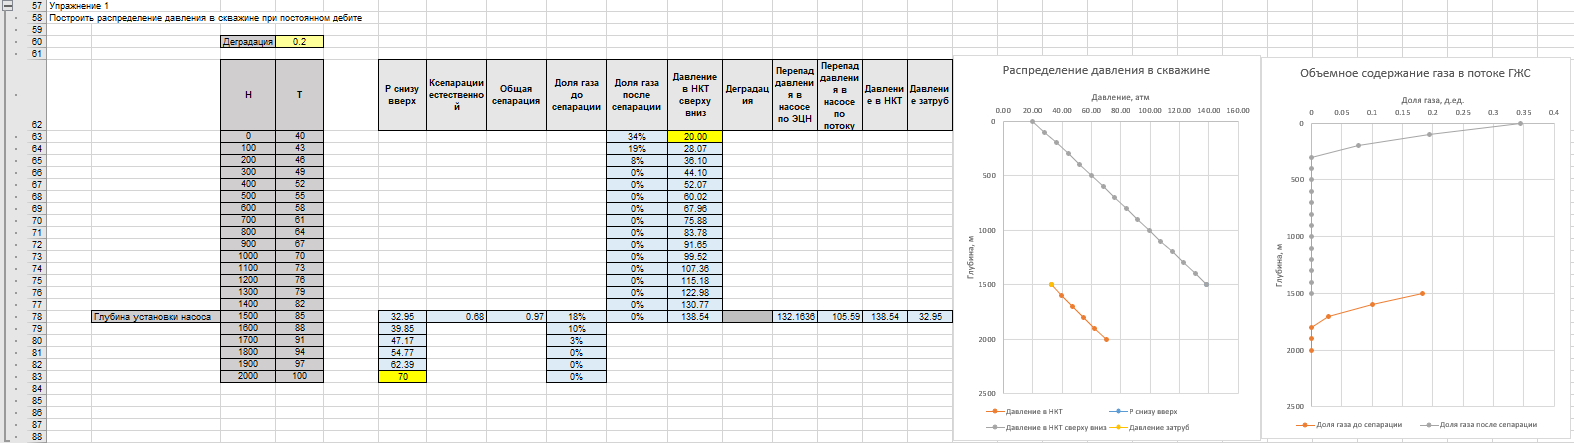
\includegraphics[width=1\linewidth]{Ex100_2}}
	\caption{Распределение давления в скважине с постоянным дебитом}
	\label{ris:Ex100_2}
\end{figure}

Во второй части упражнения распределение давления скважины строится с учетом того, что она имеет постоянную продуктивность. Изменение забойного давления в ячейке $D92$ приведет к изменению дебита скважины. Также могут варьироваться давление сепарации, коэффициент деградации и частота ЭЦН для настройки модели.

Сам расчет ведется только методом снизу-вверх: по забойному давлению определяется давление на приеме, затем вместе с коэффициентом сепарации рассчитывается перепад давления в насосе по напорной характеристике, а после устьевое давление по давлению на выходе насоса, начиная с ячейки $K114$ c помощью функции

{ \small  \texttt{=MF\_p\_pipe\_atma(Qreal\_; fw\_;C115;C114; K115;PVT\_str\_2;theta\_; Dintake\_;; D115; D114)
}}

При этом PVT строка будет использоваться другая из-за отличных значений давления на приеме по сравнению с первой частью упражнения.

\begin{figure}[h!]
	\center{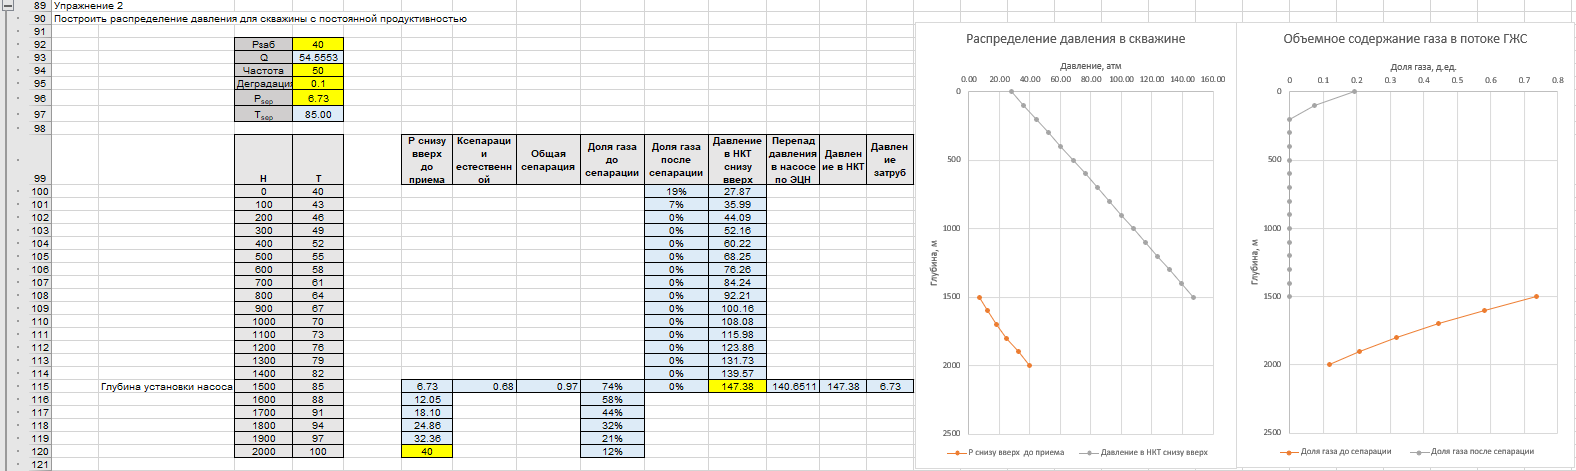
\includegraphics[width=1\linewidth]{Ex100_3}}
	\caption{Распределение давления в скважине с постоянной продуктивностью}
	\label{ris:Ex100_3}
\end{figure}

С помощью дополнительных исследований (при необходимости) ответьте на вопросы

\begin{enumerate}
	\item Как влияет сепарация, естественная и искусственная, на работу скважины?
	\item Что позволяет учесть коэффициент деградации напорной характеристики ЭЦН?
	\item Какое минимальное забойное давление можно считать оптимальным?
\end{enumerate}


\section{Анализ работы скважины, оснащенной ЭЦН, фонтанирующей через затрубное пространство}

Общая теория 

При спуске погружного оборудования в фонтанирующую скважину с большим газовым фактором газожидкостный поток у приема может разделяться на 2 составляющие: поток с низким газосодержанием после сепарации естественной и искусственной в НКТ и поток с большой долей свободного газа в затрубное пространство. 

При этом ЭЦН за счет энергии движения ГЖС работает практически на холостом ходу, развивая обычный перепад давления по напорной характеристике. Также при дебите большем, чем максимально возможный перепад давления  насоса, может происходить турбинное вращение, насос будет работать как гидравлическое сопротивление. Перегрев электродвигателя не происходит, т.к. он непрерывно охлаждается общим газожидкостным потоком.

В затрубном пространстве за счет большого количество газа будет происходить фонтанирование. Давление в затрубном пространстве будет большим, чем буферное, потому как обратный клапан в затрубе, предназначеныый для сброса газа, с жидкостью будет функционировать как штуцер, дросселируя давление. Без обратного клапана можно сделать  логичное предположение о том, что давления будут равными - газлифтный эффект в затрубном пространстве (подъем газожидкостной смеси за счет снижения плотности) будет равен перепаду давления, который создает ЭЦН.

Отсюда возникает вопрос, рационально ли устанавливать ЭЦН в фонтанирующую скважину с большим газовым фактором?

В данном упражнении предлагается смоделировать данный процесс. Но Вы также можете просмотреть расширенный расчет реальной скважины в папке "аpp".

\begin{figure}[h!]
	\center{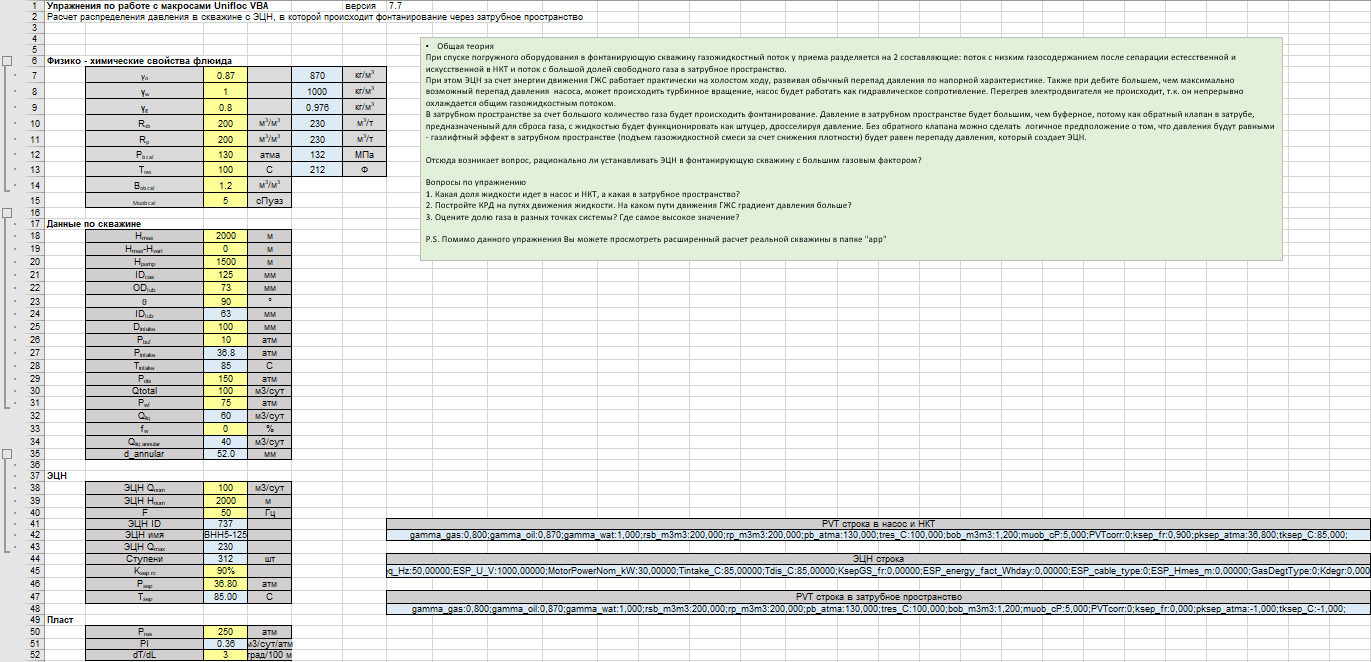
\includegraphics[width=1\linewidth]{Ex110_1}}
	\caption{Набор исходных данных, для расчета фонтанирования через затрубное пространство}
	\label{ris:Ex110_1}
\end{figure}

Процесс моделирования добывающей системы осложняется тем, что неизвестны доли жидкости: поступающая в насос и НКТ и поднимающаяся по затрубному пространству. Для этого введем коэффициент деления потока ГЖС, обозначающий долю жидкости, поступающую в насос и НКТ, в ячейке $N63$. Расчет распределения давления в НКТ и затрубном пространстве будем вести стандартным образом с помощью гидравлических корреляций. Отличия в определении давления будет выражаться в применении двух PVT строк: в ячейке $G42$ будет флюид, учитывающий сепарацию на приеме погружного оборудования, он будет описывать поведение ГЖС в НКТ, а в ячейке $G48$ будет флюид без сепарации - весь газ будет оставаться в потоке в затрубном пространстве; с помощью коэффициента деления потока из общего дебита $Q_{total}$ рассчитывается расход по НКТ $Q_{liq}$ и по затрубному  пространству $Q_{liq annular}$

К формулам, используемым в предыдущем упражнении, добавляется расчет давления в затрубном пространстве (с $Q80$)

{ \small  \texttt{=MF\_p\_pipe\_atma(Q\_annular\_; fw\_; C81;C80; Q81; PVT\_str\_annular\_; theta\_; d\_annular\_pr; 1;D81;D80)
}}

И соответственно доля газа в ГЖС затрубного пространства (с $J81$) 

{ \small  \texttt{=MF\_gas\_fraction\_d(Q81; D81; fw\_; PVT\_str\_annular\_)
}}

Также напомним о важности правильно определения давления сепарации (описано выше). 

Таким образом, с помощью КРД в затрубном пространстве и НКТ предлагается найти такие параметры системы (изменяя коэффициент деления потока, коэффициент деградации напорной характеристики насоса и т.д.) при котором давление в затрубном пространстве будет равным или большим, чем буферное давление.

\begin{figure}[h!]
	\center{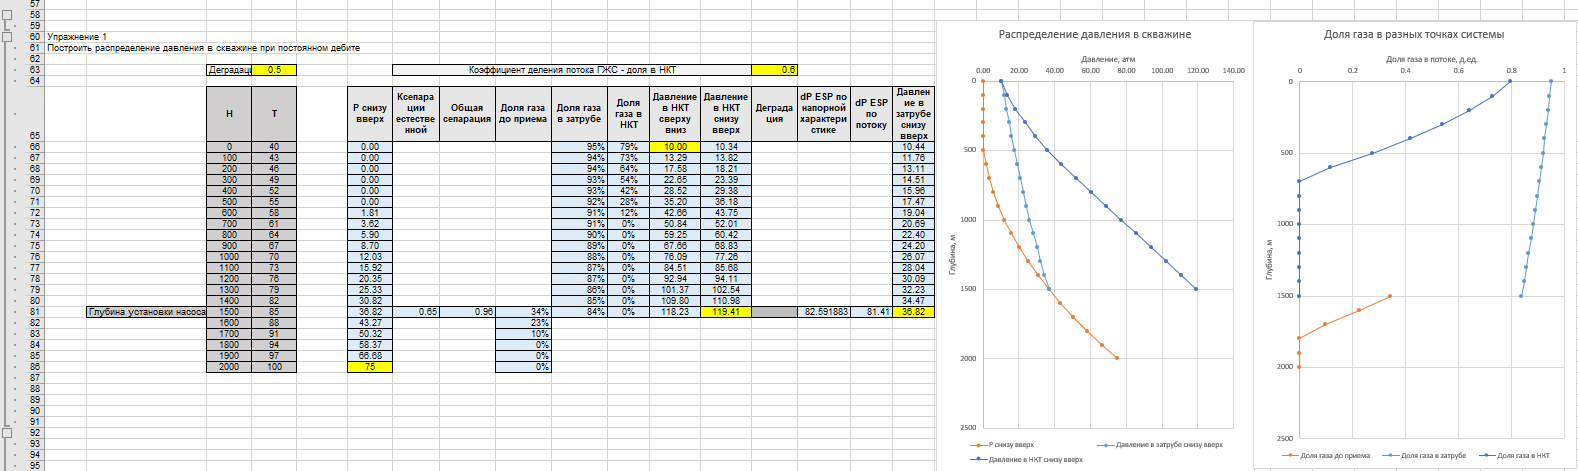
\includegraphics[width=1\linewidth]{Ex110_2}}
	\caption{Настроенная модель скважины с равными давлениями на устье}
	\label{ris:Ex110_2}
\end{figure}

Вопросы по упражнению
\begin{enumerate}
	\item  Какая доля жидкости идет в насос и НКТ, а какая в затрубное пространство?
	\item  Постройте КРД на путях движения жидкости. На каком пути движения ГЖС градиент давления больше?
	\item Оцените долю газа в разных точках системы? Где самое высокое значение?
	\item Оптимальнее ли будет эксплуатировать скважину с помощью чисто фонтанного способа добычи?
\end{enumerate}


\section{Набор расчетных модулей анализа скважины}
Пример использования алгоритмов \unf   приведен в файле \texttt{UF7\_calc\_well.xlsm}.

Файл содержит набор расчетных модулей позволяющих провести анализ данных описывающих работу скважины с применением различных методов добычи.

\subsection{Расчетный модуль анализа и настройки PVT свойств}

